% #############################################################################
% This is Chapter 4
% !TEX root = ../main.tex
% #############################################################################
% Change the Name of the Chapter i the following line
\fancychapter{Conducted Numerical Simulations}
% \cleardoublepage
% The following line allows to ref this chapter
\label{chap:implement}

\section{Dirac equation simulations}

Recall the system of equations given in \eqref{dirac}
\begin{equation}
    \begin{bmatrix}
        m & -i(\partial_1 - i \partial_2)\\
        -i(\partial_1 + i \partial_2) & -m
    \end{bmatrix}
    \begin{bmatrix}
        u_1(x)\\
        u_2(x)
    \end{bmatrix}
    =\lambda
    \begin{bmatrix}
    u_1(x)\\
    u_2(x)
    \end{bmatrix},
\end{equation}
which can be reduced to the Helmholtz equation with Cauchy-Riemann oblique boundary conditions
\begin{equation*}
    \begin{cases}
        &-\Delta u_1 = (\lambda^2 - m^2)u_1, \; \text{ in } \Omega\\
        & i (\partial_1 + i\partial_2)u_1 + (\lambda + m)i(n_1 + i n_2)u_1 = 0, \; \text{ on } \Gamma,
    \end{cases}      
\end{equation*}
where \(\Gamma = \partial\Omega\) as usual, and the function \(u_2\) depends on the function \(u_1\) by the following equality
\[
    u_2 = \frac{-i (\partial_1 + i\partial_2)u_1}{\lambda + m}.    
\]
\subsection{Method validation}

In order to validate the method of fundamental solutions, we start by testing it for the unit disk. If \(m=0\), then its value is known, like stated in Proposition \ref{dirac_properties}, where \(\lambda_1(\mathbb{D})= 1.434695650819\) is the solution of the equation
\[
    J_0(\lambda_1(\mathbb{D})) = J_1(\lambda_1(\mathbb{D})).
\]

In the numerical simulations presented below, 158 inner collocation points for the subspace angle technique were considered and the number of source points \(N\) is always half of the number of boundary points. Figure \ref{dirak_disk_col_m0} shows the configuration used. The method described at the end of the subchapter \ref{density_proofs_section} was used to place the source points, where \(\eta=0.5\) was used. 

\begin{figure}[!htb]
    \centering
    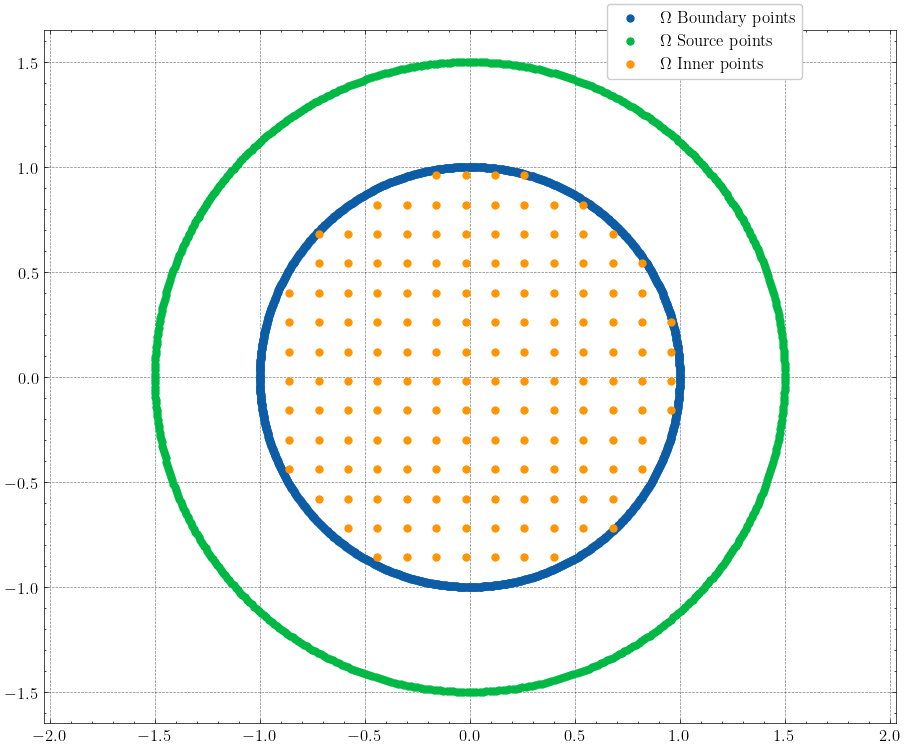
\includegraphics[width=0.5\linewidth]{Images/Dirac/circle_m_0_col_points_158_inner_eta_05.png}
    \captionof{figure}{Configuration of the boundary, source and inner points. The number of boundary collocation points used is 1200.}
    \label{dirak_disk_col_m0}
\end{figure}

While in the other numerical simulations to be presented more eigenvalues are studied, in Table \ref{tab:eigenvalues_disk_val} only the first three eigenvalues are shown for sake of brevity.

\begin{table}[htbp]
    \centering
    \begin{tabular}{cccc}
        \toprule
        \textbf{Eigenvalues} & \textbf{N=1200} & \textbf{N=1000} & \textbf{N=800} \\
        \midrule
        \(\tilde{\lambda}_1(\mathbb{D})\) & $1.4346956515$ & $1.4346956481$ & $1.4346956367$ \\
        \(\tilde{\lambda}_2(\mathbb{D})\) & $2.6298741163$ & $2.6298741147$ & $2.6298741276$ \\
        \(\tilde{\lambda}_3(\mathbb{D})\) & $3.1128644920$ & $3.1128645083$ & $3.1128645008$ \\
        \midrule
        \textbf{Absolute error: } \(\abs{\lambda_1(\mathbb{D}) - \tilde{\lambda}_1(\mathbb{D})}\) & $6,877\times 10^{-10}$ & $2,693\times 10^{-9}$ & $1,413\times 10^{-8}$ \\
        \bottomrule
    \end{tabular}
    \caption{Eigenvalues for different values of \(N\) and the measured absolute error.}
    \label{tab:eigenvalues_disk_val}
\end{table}

The plot of the bracketing algorithm \ref{direct_bracketing_algorithm} is shown in Figure \ref{dirac_disk_alg_m0}. For future reference, the first eigenfunction on the disk with \(m=0\) is also shown in Figure \ref{dirac_disk_plots_m0}, where the real and imaginary parts of the spinors \(u_1\) and \(u_2\) are presented. The plots are also normalized, i.e, \(\norm*{\mathbf{u}}_{L^2(\mathbb{D})}=1\).

\begin{figure}[!htb]
    \centering
    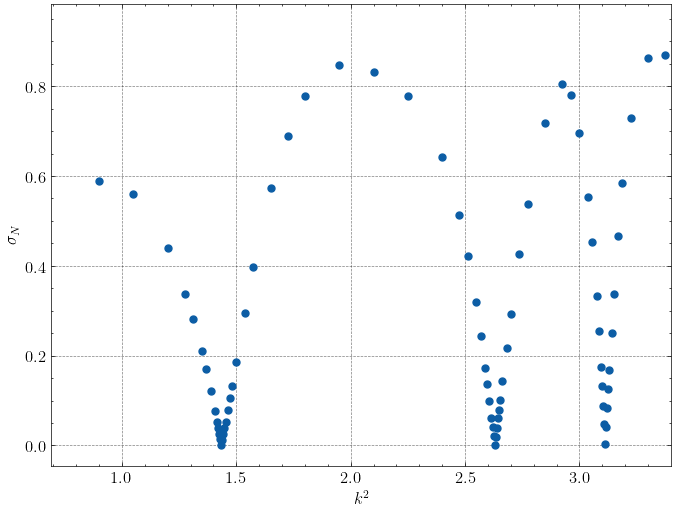
\includegraphics[width=0.5\linewidth]{Images/Dirac/circle_m_0_alg_points_158_inner_eta_05.png}
    \captionof{figure}{Direct search algorithm for the first three eigenvalues of the disk with \(m=0\). Empirically, better approximations are obtained when smaller values of \(\sigma_N\) are found in each singularity.}
    \label{dirac_disk_alg_m0}
\end{figure}

\begin{figure}[!htb]
    \centering
    \begin{minipage}[b]{0.45\textwidth}
        \centering
        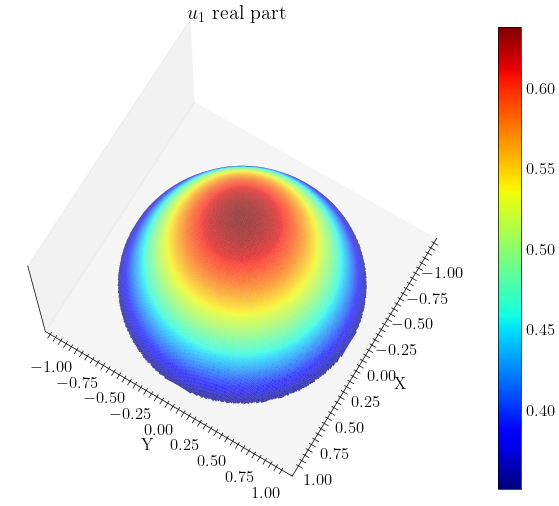
\includegraphics[width=0.8\textwidth]{Images/Dirac/circle_m_0_u1_re_points_158_inner_eta_05.png}
%\caption{Network 1}
    \end{minipage}
    \hfill
    \begin{minipage}[b]{0.45\textwidth}
        \centering
        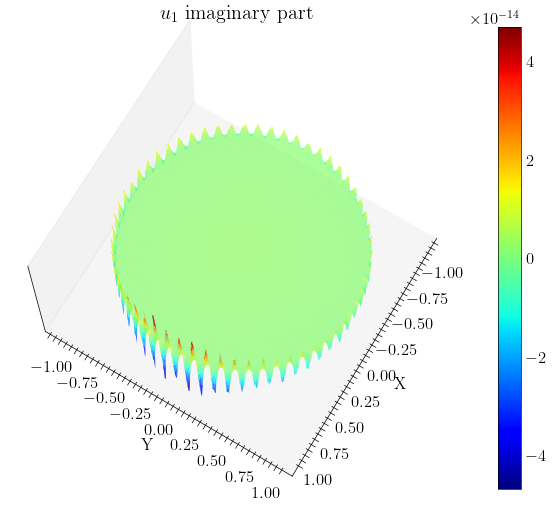
\includegraphics[width=0.8\textwidth]{Images/Dirac/circle_m_0_u1_im_points_158_inner_eta_05.png}
%\caption{Network 2}
    \end{minipage}

    \vspace{0.5cm}

    \begin{minipage}[b]{0.45\textwidth}
        \centering
        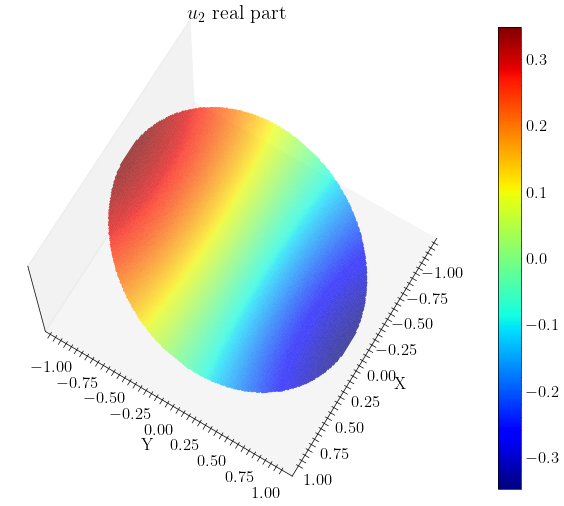
\includegraphics[width=0.8\textwidth]{Images/Dirac/circle_m_0_u2_re_points_158_inner_eta_05.png}
%\caption{Network 3}
    \end{minipage}
    \hfill
    \begin{minipage}[b]{0.45\textwidth}
        \centering
        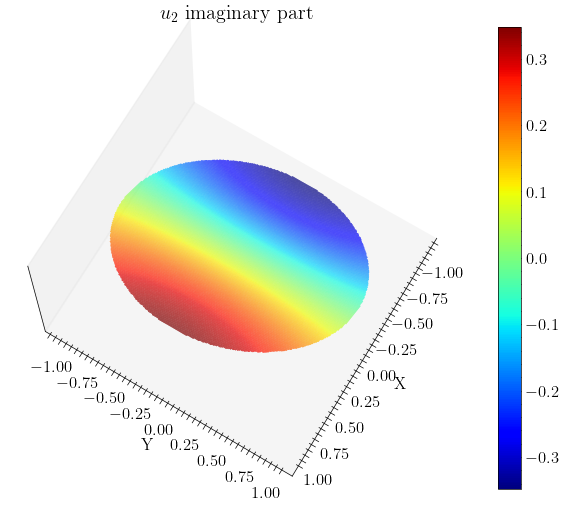
\includegraphics[width=0.8\textwidth]{Images/Dirac/circle_m_0_u2_im_points_158_inner_eta_05.png}
%\caption{Network 4}
    \end{minipage}
    \caption{Plots of the real and imaginary parts of \(u_1\) and \(u_2\) of the first eigenfunction \(\mathbf{u}=\begin{bmatrix} u_1\\ u_2 \end{bmatrix}\). Observe that the imaginary part of \(u_1\) is zero and the artifacts presented are due to precision lost.}
    \label{dirac_disk_plots_m0}
\end{figure}



\subsection{Quadrilateral results}

In this subsection several results numerical regarding quadrilateral polygons are shown and discussed. First, numerical evidence for Conjecture \ref{david_conjectures} is presented both for \(m=1\) and \(m=5\). Then, some simulations show that an analogous to the Ashbaugh-Benguria inequality \ref{ashbaugh-benguria theorem} for the Laplace operator also holds for the Dirac Operator with infinite-mass boundary conditions. Finally, we will also show that similarities between the spectrum of both operators are already evident for the third eigenvalue, whose optimal shape is not the disk, contrary to what is conjectured for the Laplacian (which is still an open problem).

Consider a rectangle with a width \(a > 0\) and unitary area, where the sides are \(a\) and \(\frac{1}{a}\). Figures \ref{eigenvalues_rectangle_width_m_1} and \ref{eigenvalues_rectangle_width_m_5} illustrate the behavior of the first 5 eigenvalues for \(m=1\) and \(m=5\), respectively. Several interesting observations can be made:

\begin{itemize}
  \item The behavior of the spectrum remains qualitatively consistent for different values of \(m\). Notably, the most prominent difference lies in the decreasing gap between the numerical eigenvalues and \(m\) as \(m\) increases. While this trend is discernible, it becomes more apparent as \(m\) takes on even larger values;
  
  \item Starting from the third eigenvalue and beyond, certain spikes become evident in the plot. These spikes correspond to rectangular domains where the eigenvalue has multiplicity two. For instance, between the values 1 and 1.5, the third and fourth eigenvalues appear to converge. This behavior becomes more frequent as the order of the eigenvalues increases. However, only multiplicity 2 is observed which is not consistent with the behavior seen in the Laplace operator, where multiplicity 3 is already achieved in the third eigenvalue and only the first eigenvalue is simple;
  
  \item By varying the parameter \(a\), a linear growth in the eigenvalues is observed, with no change in their multiplicity. As \(a\) increases, the eigenvalues approach one another, as expected. This phenomenon occurs because the rectangle transforms into an unbounded line, resulting in a non-discrete spectrum.
\end{itemize}

\begin{figure}[!htb]
    \centering
    \begin{minipage}{.5\textwidth}
      \centering
      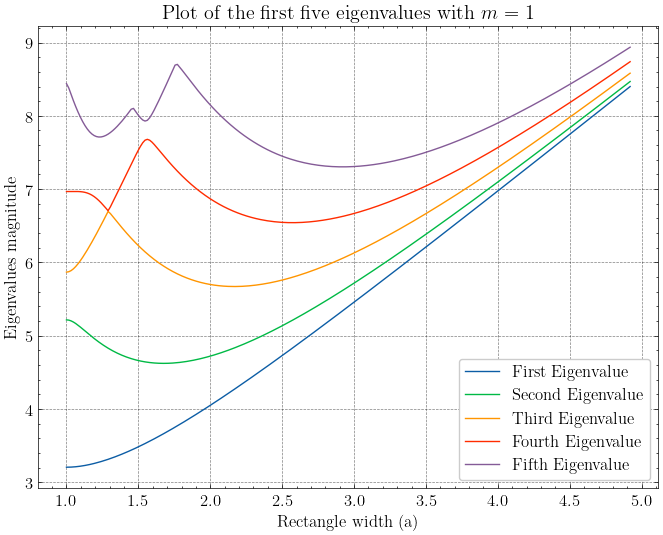
\includegraphics[width=\linewidth]{Images/Dirac/quad/eigenvalues_rectangle_width_m_1.png}
      \captionsetup{width=0.9\linewidth} % Adjust the width of the caption
      \captionof{figure}{Behavior of the first five eigenvalues for rectangles with unit area, width \(a\) and \(m=1\).}
      \label{eigenvalues_rectangle_width_m_1}
    \end{minipage}%
    %\hspace{0.5cm} % Add some horizontal space between the figures
    \begin{minipage}{.5\textwidth}
      \centering
      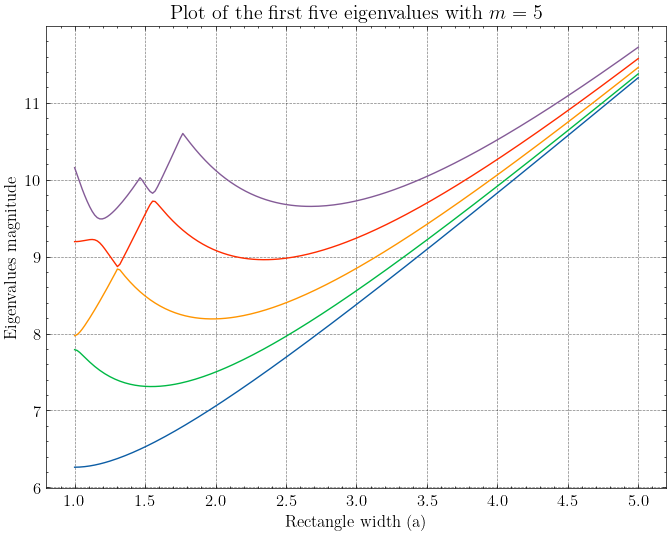
\includegraphics[width=1\linewidth]{Images/Dirac/quad/eigenvalues_rectangle_width_m_5.png}
      \captionsetup{width=0.9\linewidth} % Adjust the width of the caption
      \captionof{figure}{Behavior of the first five eigenvalues for rectangles with unit area, width \(a\) and \(m=5\).}
      \label{eigenvalues_rectangle_width_m_5}
    \end{minipage}
\end{figure}

In Figures \ref{eigenvalues_rectangle_perimeter_width_m_1} and \ref{eigenvalues_rectangle_perimeter_width_m_5} the results for the perimeter are shown. While Conjecture \ref{david_conjectures} is framed for \(a \in (0, 2)\) observe that is enough to consider \(a \in (0, 1)\) given the symmetry of the problem. Here, one considers the perimeter to be 4 and by varying the rectangle width the area is not constant. The conclusions presented earlier are still valid.

\begin{figure}[!htb]
    \centering
    \begin{minipage}{.5\textwidth}
      \centering
      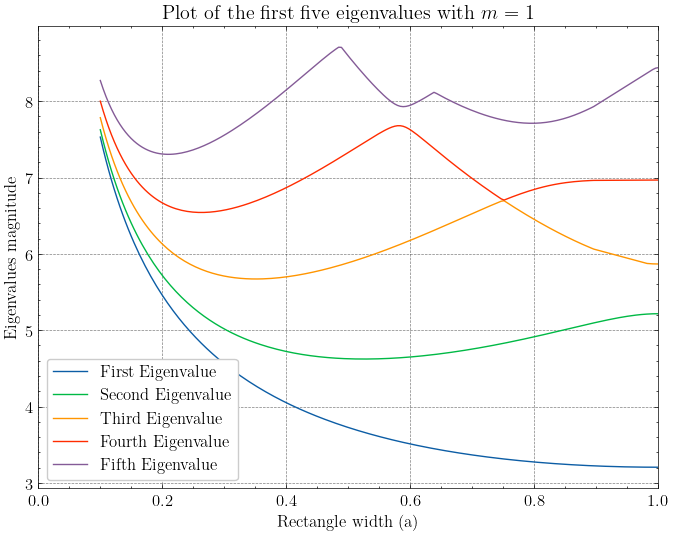
\includegraphics[width=\linewidth]{Images/Dirac/quad/eigenvalues_rectangle_perimeter_width_m_1.png}
      \captionsetup{width=0.9\linewidth} % Adjust the width of the caption
      \captionof{figure}{Behavior of the first five eigenvalues for rectangles with unit area, width \(a\) and \(m=1\).}
      \label{eigenvalues_rectangle_perimeter_width_m_1}
    \end{minipage}%
    %\hspace{0.5cm} % Add some horizontal space between the figures
    \begin{minipage}{.5\textwidth}
      \centering
      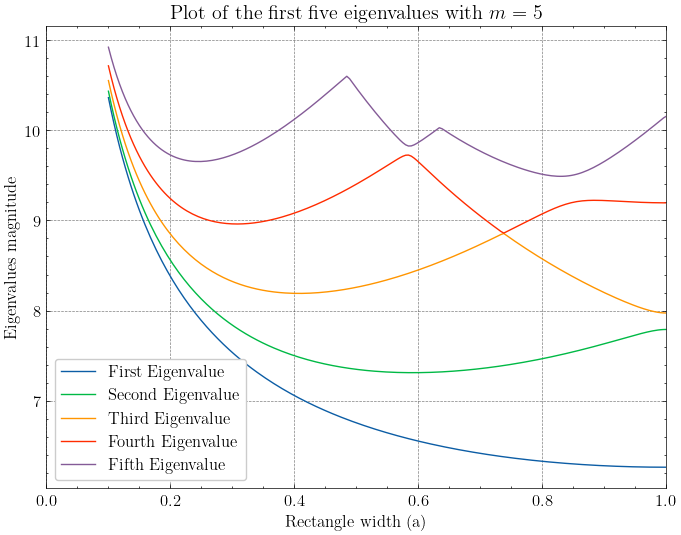
\includegraphics[width=1\linewidth]{Images/Dirac/quad/eigenvalues_rectangle_perimeter_width_m_5.png}
      \captionsetup{width=0.9\linewidth} % Adjust the width of the caption
      \captionof{figure}{Behavior of the first five eigenvalues for rectangles with unit area, width \(a\) and \(m=5\).}
      \label{eigenvalues_rectangle_perimeter_width_m_5}
    \end{minipage}
\end{figure}

Given the results for rectangles with fixed area or perimeter, it is possible to state that the Conjecture \ref{david_conjectures} should hold, although it is still not possible ascertain that the results presented here hold for every \(m\). In any case, it is known that the eigenvalues are continuous with domain perturbations (here these perturbations can be seen as stretching the rectangles), exactly what has been found in these numerical simulations.

To finish this subsection, we present the results for general quadrilaterals. Since there is no (practical) parameterization which can describe every quadrilateral, we have resorted to random sampling of quadrilaterals and study the results against rectangles and rhombus. Figure \ref{dirac_first_three_eigenvalues_quad_m_1} presents the results of the numerical simulations for \(m=1\). Notice how the rectangles and rhombus clearly define a region of ``acceptable'' quadrilaterals and this is appears to be particularly true for the first eigenvalue. For the second and third eigenvalues some quadrilaterals behave differently, and it is already possible find some domains whose third eigenvalue is smaller than the eigenvalue of the unit disk. In Figures \ref{dirac_benguria_quad} and \ref{dirac_generalized_benguria_quad} the ratio between the first eigenvalues is studied, where a version of the Ashbaugh-Benguria Theorem \ref{ashbaugh-benguria theorem} appears to hold.

\begin{figure}[!htb]
    \centering
    \begin{minipage}[c]{0.8\textwidth}
        \centering
        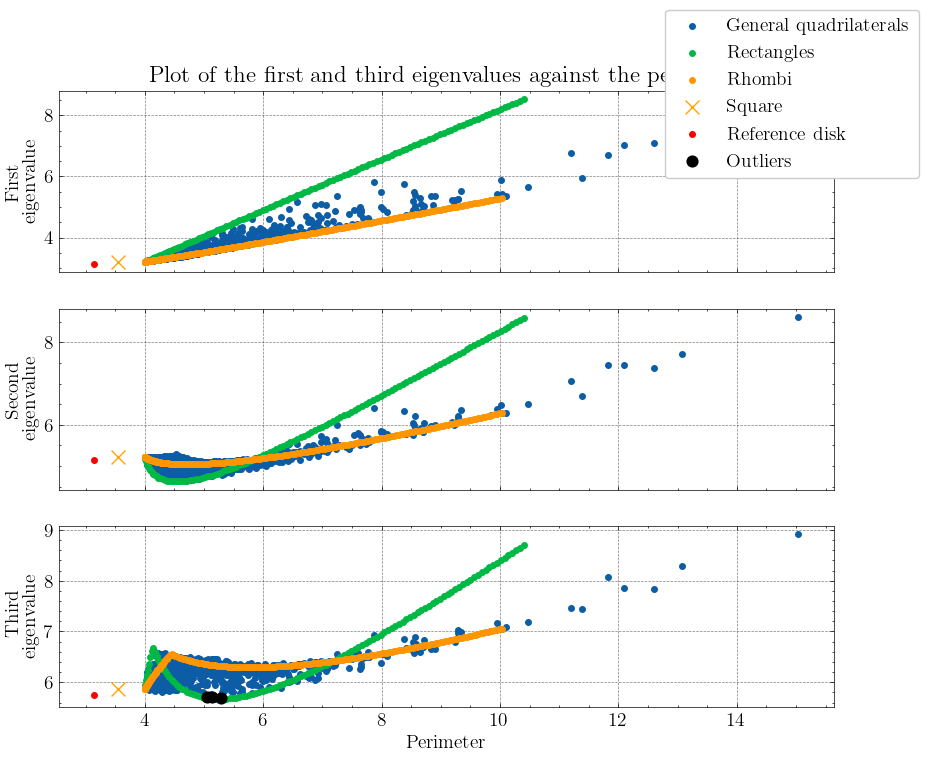
\includegraphics[width=0.8\textwidth]{Images/Dirac/quad/first_three_eigenvalues_quad_m_1.png}
        \caption{Plot of the first three eigenvalues against the perimeter. The ``outliers'' marked in black represent the domains in which the third eigenvalue is less that the third eigenvalue of the disk.}
        \label{dirac_first_three_eigenvalues_quad_m_1}
    \end{minipage}

    \vspace{0.5cm}

    \begin{minipage}[c]{0.41\textwidth}
        \centering
        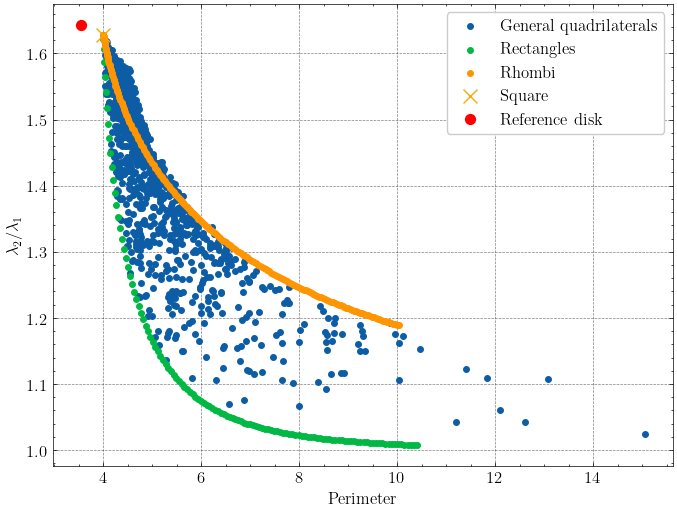
\includegraphics[width=\textwidth]{Images/Dirac/quad/benguria_quad.png}
        \captionsetup{width=0.8\linewidth} % Adjust the width of the caption
        \caption{Ratio between the first two eigenvalues \(\frac{\lambda_2}{\lambda_1}\).}
        \label{dirac_benguria_quad}
    \end{minipage}
    \hfill
    \begin{minipage}[c]{0.50\textwidth}
        \centering
        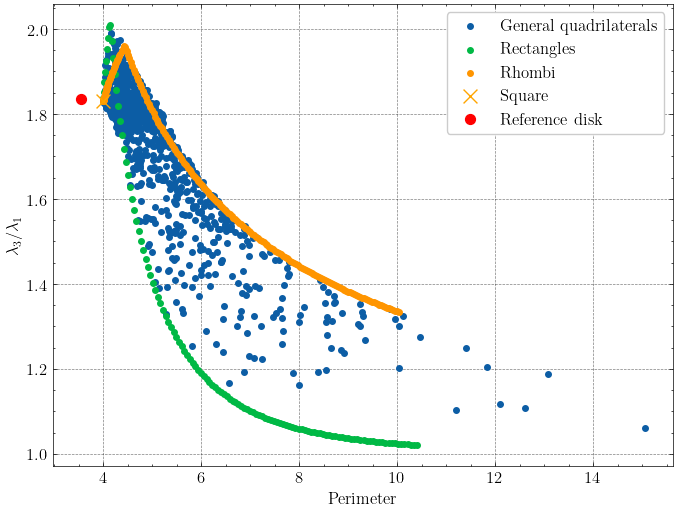
\includegraphics[width=\textwidth]{Images/Dirac/quad/generalized_benguria_quad.png}
        \captionsetup{width=0.8\linewidth} % Adjust the width of the caption
        \caption{Ratio between the third and first eigenvalues \(\frac{\lambda_3}{\lambda_1}\).}
        \label{dirac_generalized_benguria_quad}
    \end{minipage}
    \vspace{0.5cm}
\end{figure}

\subsection{Triangle results}

In this subsection we tackle the Conjectures \ref{triangle_conjectures} stated on \cite{vu2023spectral}. Instead of considering random triangles, its study can be done systematically given that, up to congruence, three parameters completely define every triangle. The approach presented here is based on the work of Antunes \& Freitas \cite{antunes2011inverse}. Consider the region \(R\) defined by
\[
    R = \{(x, y) \in \mathbb{R}^2: x \geq 0, y > 0, (x+1)^2 + y^2 \leq 4\},
\]
and its piecewise boundary \(\partial R = \Gamma_0 \cup \Gamma_1 \cup \Gamma_2\), where
\begin{align*}
    \Gamma_0 &= \{(x,y) \in \mathbb{R}^2: 0 \leq x \leq 1, y=0\}\\
    \Gamma_1 &= \{(x,y) \in \mathbb{R}^2: 0 \leq x < 1, y=\sqrt{4-(x+1)^2}\}\\
    \Gamma_2 &= \{(x,y) \in \mathbb{R}^2: x=0, 0 < y < \sqrt{3}\}.
\end{align*}
A triangle \(T\) is said to be \textit{admissible}\footnote{Of course, one does not need to enforce such constraints to triangle: as said before, every triangle is unique up to congruence. Here, we just emphasize that is enough to consider triangles defined using the region \(R\). Observe that this is just a model to numerically exhaust all possible triangles up to congruence, one still needs to normalize them to have unitary area.} if its basis vertices are \((0, 0\)) and \((1, 0)\), and the other vertex coordinates are \((x,y)\) such that \((x,y) \in \overline{R}\). A triangle \(T\) is said to be \textit{subequilateral} if \((x, y) \in \Gamma_1\) and \textit{superequilateral} if \((x, y) \in \Gamma_2\); if \((x, y) = (0, \sqrt{3})\) then it is equilateral (obviously). The plot of the region \(R\) and its boundary \(\partial R\) is in Figure \ref{dirac_triangle_model}.
\begin{figure}[!htb]
    \centering
    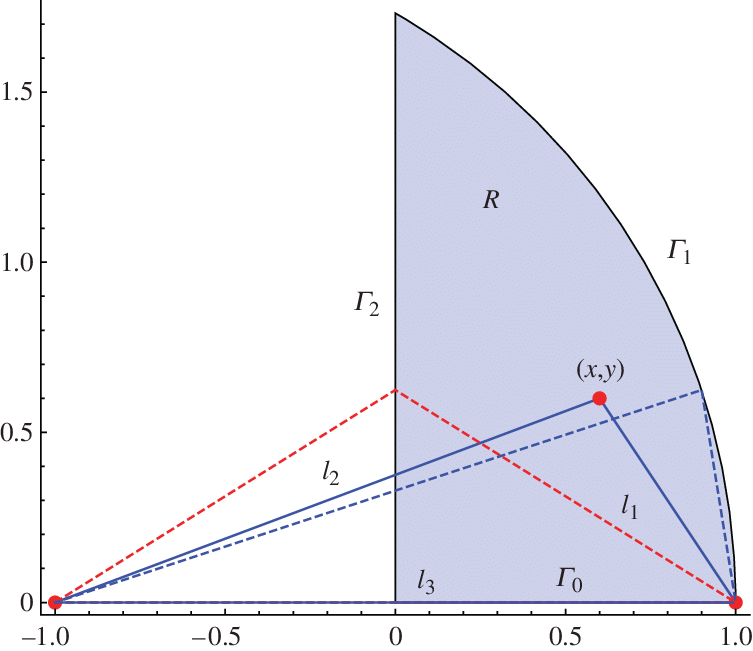
\includegraphics[width=0.5\linewidth]{Images/Dirac/model_triangle.png}
    \captionof{figure}{Configuration space of the admissible triangles. In a dashed red line is a superequilateral triangle; in a dashed blue line a subequilateral triangle is also represented.}
    \label{dirac_triangle_model}
\end{figure}
In Figure \ref{dirac_smooth_first_eigenvalues} we present numerical evidence for Conjecture \ref{triangle_conjectures} with \(m=1\). Notice how the eigenvalues of the superequilateral and subequilateral triangles define a region that includes every other triangle whose \((x, y)\) vertex belongs to \(R\). In Figure \ref{dirac_triangle_benguria} a version of the Ashbaugh-Benguria (see Theorem \ref{ashbaugh-benguria theorem}) inequality is presented and in Figure \ref{dirac_triangle_3d_lambda1} a 3D plot of the first eigenvalue for every admissible triangle considered against the coordinates \((x,y)\) of the vertex in \(\overline{R}\).

\begin{figure}[!htb]
    \centering
    \begin{minipage}[c]{0.8\textwidth}
        \centering
        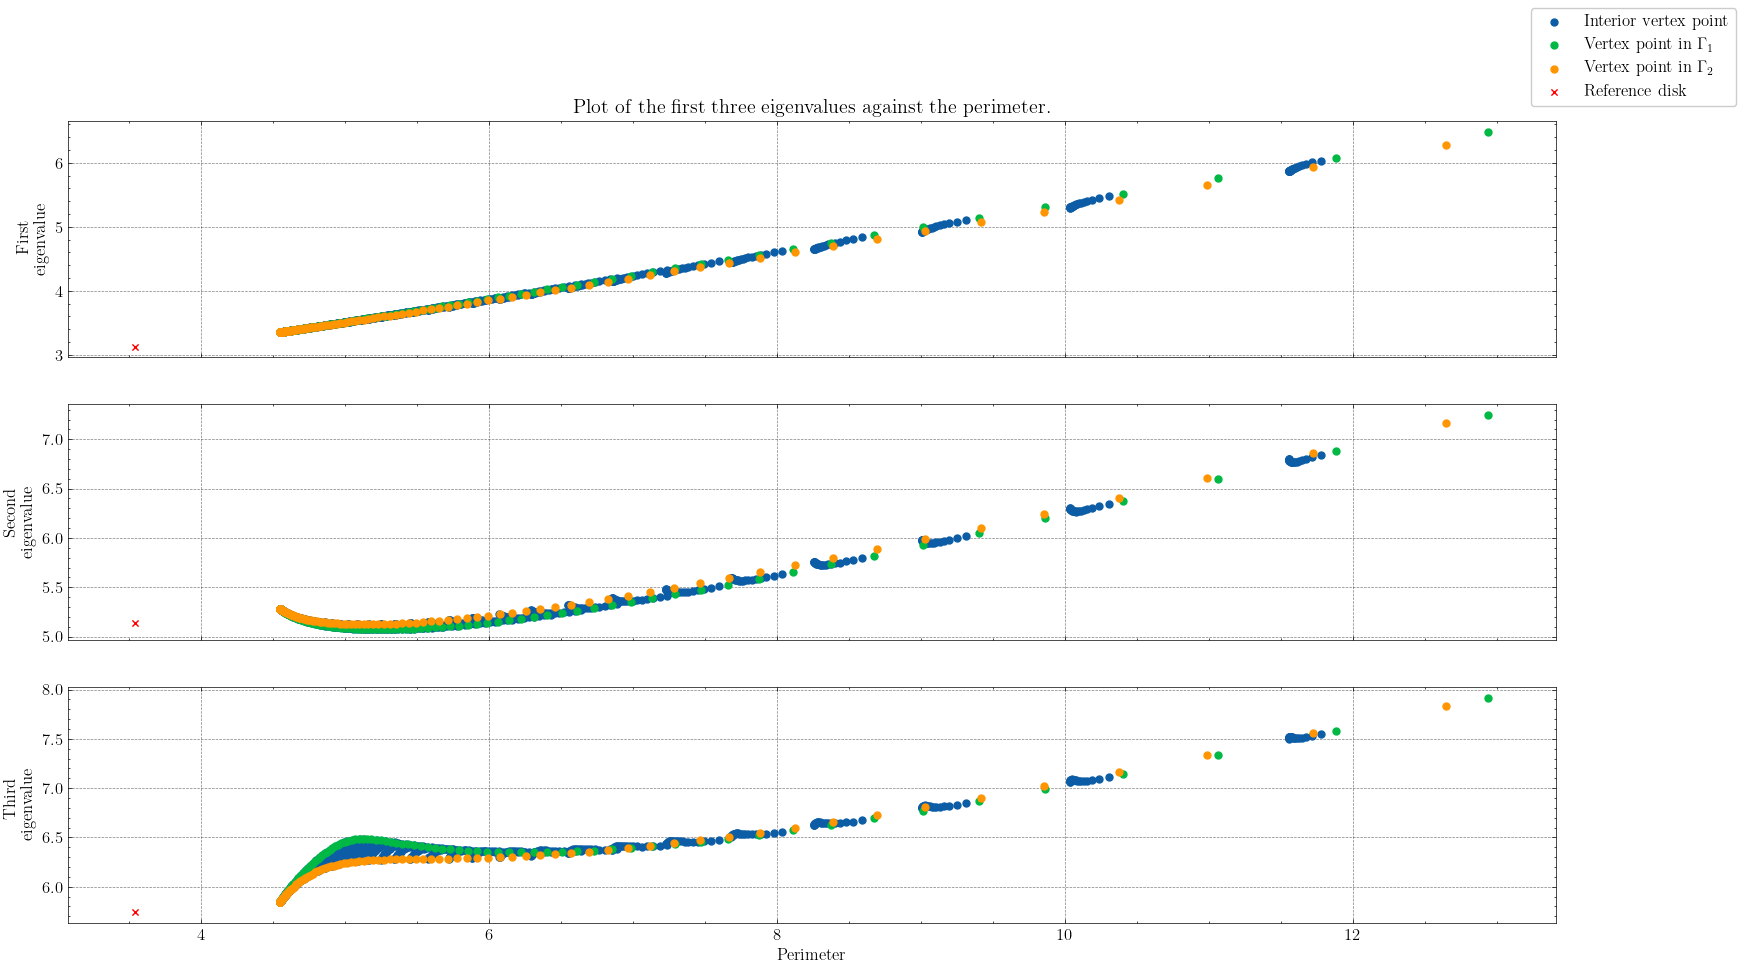
\includegraphics[width=\textwidth]{Images/Dirac/triangles/triangle_first_eigenvalues.png}
        \caption{Plot of the first three eigenvalues against the perimeter. The ``outliers'' marked in black represent the domains in which the third eigenvalue is less that the third eigenvalue of the disk.}
        \label{dirac_smooth_first_eigenvalues}
    \end{minipage}

    \vspace{0.5cm}

    \begin{minipage}[c]{0.41\textwidth}
        \centering
        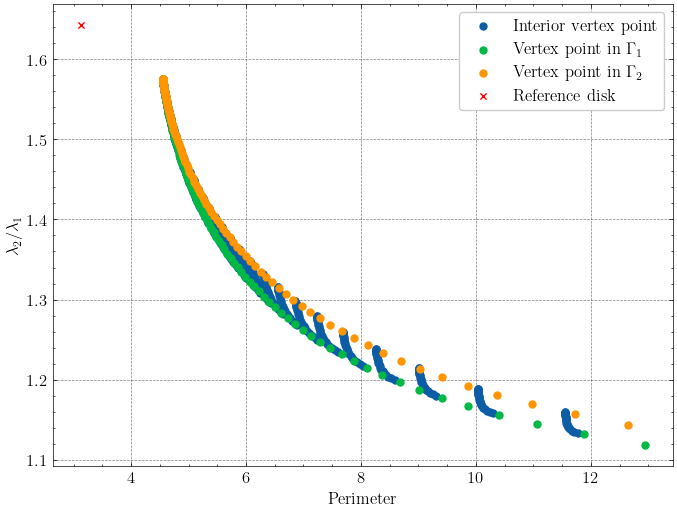
\includegraphics[width=\textwidth]{Images/Dirac/triangles/triangle_benguria.png}
        \captionsetup{width=0.8\linewidth} % Adjust the width of the caption
        \caption{Ratio between the first two eigenvalues \(\frac{\lambda_2}{\lambda_1}\).}
        \label{dirac_triangle_benguria}
    \end{minipage}
    \hfill
    \begin{minipage}[c]{0.50\textwidth}
        \centering
        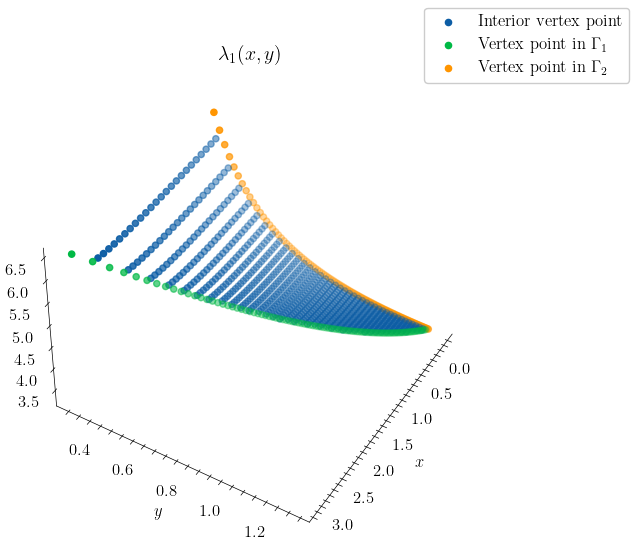
\includegraphics[width=\textwidth]{Images/Dirac/triangles/triangle_3d_lambda1.png}
        \captionsetup{width=0.8\linewidth} % Adjust the width of the caption
        \caption{Ratio between the third and first eigenvalues \(\frac{\lambda_23}{\lambda_1}\).}
        \label{dirac_triangle_3d_lambda1}
    \end{minipage}
    \vspace{0.5cm}
\end{figure}

While in the previous results for quadrilaterals (and for smooth domains in the next subsection) random domains were considered, it is remarkable that for the triangle problem one can consider \textit{every} type of triangle just by varying \((x,y)\) in \(\overline{R}\). Since the eigenvalues are continuous when considering domain perturbations, it means that it is very unlikely that the conjectures studied for triangles do not hold, otherwise some jump would probably be found, for example in Figure \ref{dirac_triangle_3d_lambda1}. 


\subsection{Smooth domain results}

In this last subsection, the behavior of the spectrum for smooth (connected) domains with unitary area is studied. Here, we fix \(m=1\). The objective of this study is twofold: first, this type of domains is studied since the numerical approximations are more reliable, and it allows for the study of arbitrary domains; second, one can use them to also study the domain which minimizes the third eigenvalue.

In order to generate random smooth domains, periodic B-spline interpolation for each component of an \(\mathbb{R}^2\) vector was used. One starts by generate five random points (using a uniform distribution), fit a periodic B-spline in each component, draw the two-dimensional B-spline and check for auto-intersections. If it does not auto-intersect, then it is a valid domain. Figure \ref{dirac_smooth_random_domain} presents one of these type of domains.

\begin{figure}[!htb]
    \centering
    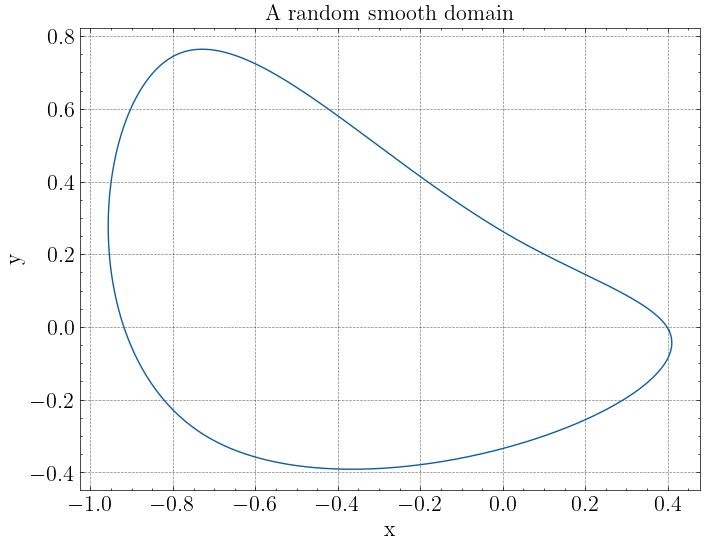
\includegraphics[width=0.55\linewidth]{Images/Dirac/smooth/random_smooth_domain.png}
    \captionof{figure}{Some smooth domain generated by B-splines.}
    \label{dirac_smooth_random_domain}
\end{figure}

Figures below are analogous to the ones presented before. In Figure \ref{dirac_smooth_domains_scatter_all_eigs} a scatter plot of the first three eigenvalues as a function of the perimeter. Once again, analogously to the Laplacian, a Faber-Krahn type result appears to hold for the Dirac operator with infinite-mass boundary conditions. As we saw before, some ``outlier'' domains have a third eigenvalue which is smaller than the third eigenvalue on the disk, which contradicts the conjecture for the Laplace operator.
In Figures \ref{dirac_smooth_domains_scatter_benguria}, \ref{dirac_smooth_domains_scatter_benguria_third} are related to the ratio of the first eigenvalues and the spectral gap between them. An analogous to the Ashbaugh-Benguria Theorem for the Laplacian also seems to hold for the Dirac operator, as well its generalization for the ratio \(\frac{\lambda_3}{\lambda_1}\).

\begin{figure}[!htb]
    \centering
    \begin{minipage}[c]{0.8\textwidth}
        \centering
        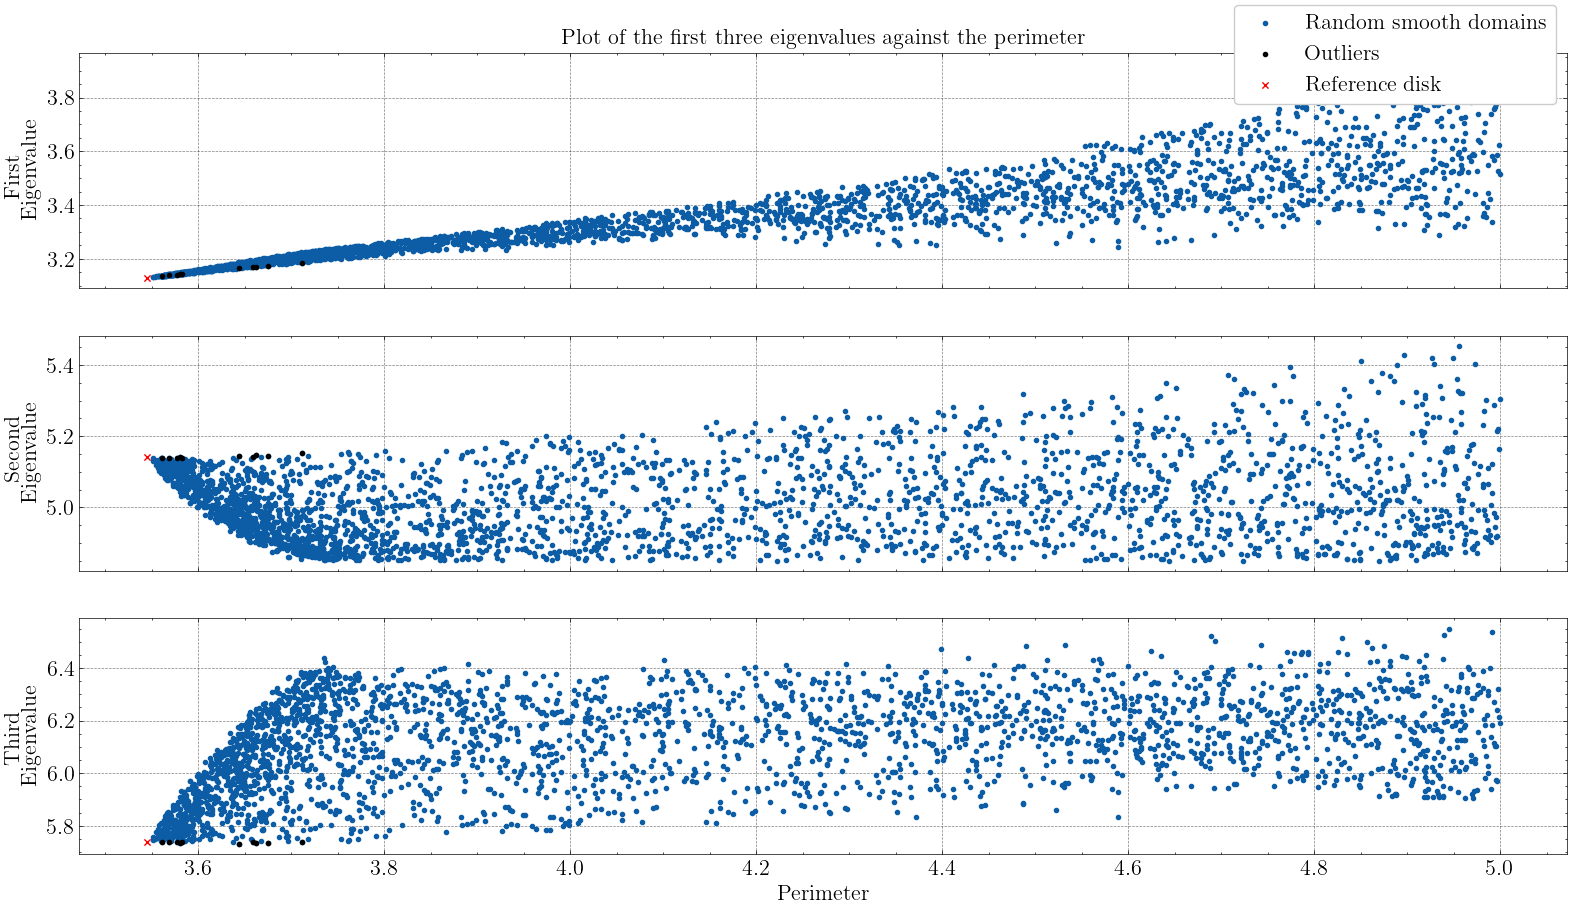
\includegraphics[width=\textwidth]{Images/Dirac/smooth/smooth_domains_scatter_all_eigs_.png}
        \caption{Plot of the first three eigenvalues against the perimeter. The ``outliers'' marked in black represent the domains in which the third eigenvalue is less that the third eigenvalue of the disk.}
        \label{dirac_smooth_domains_scatter_all_eigs}
    \end{minipage}

    \vspace{0.5cm}

    \begin{minipage}[c]{0.45\textwidth}
        \centering
        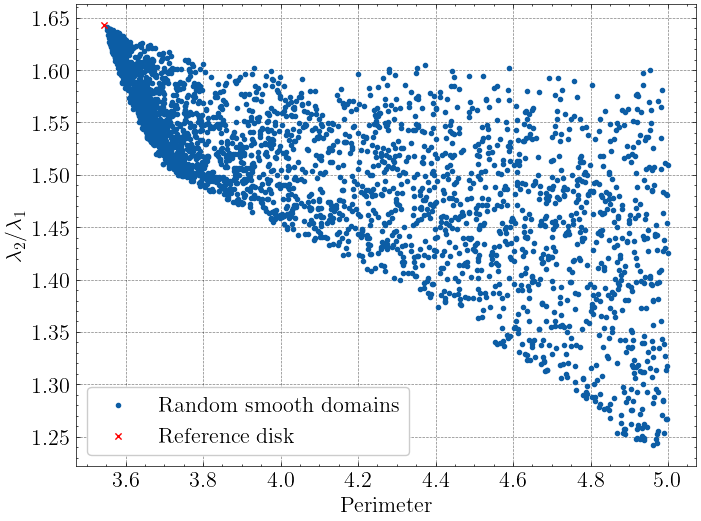
\includegraphics[width=\textwidth]{Images/Dirac/smooth/smooth_domains_scatter_benguria.png}
        \caption{Ratio between the first two eigenvalues \(\frac{\lambda_2}{\lambda_1}\).}
        \label{dirac_smooth_domains_scatter_benguria}
    \end{minipage}
    \hfill
    % \begin{minipage}[c]{0.32\textwidth}
    %     \centering
    %     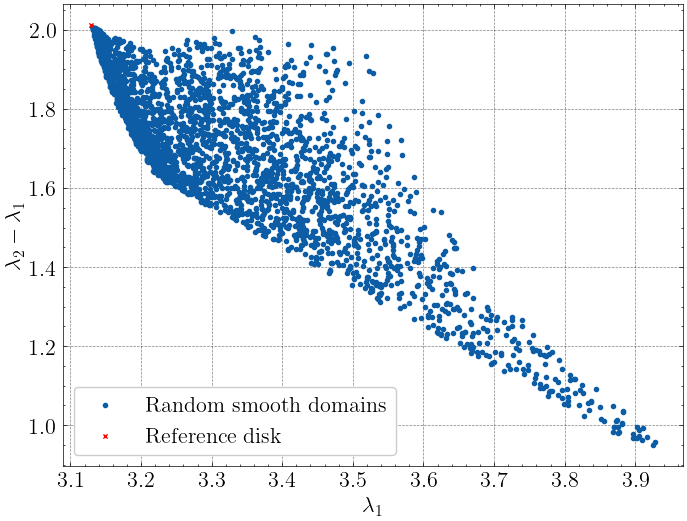
\includegraphics[width=\textwidth]{Images/Dirac/smooth/smooth_domains_scatter_gap.png}
    %     \caption{Spectral gap \(\lambda_2-\lambda_1\).}
    %     \label{dirac_smooth_domains_scatter_gap}
    % \end{minipage}
    % \hfill
    \begin{minipage}[c]{0.45\textwidth}
        \centering
        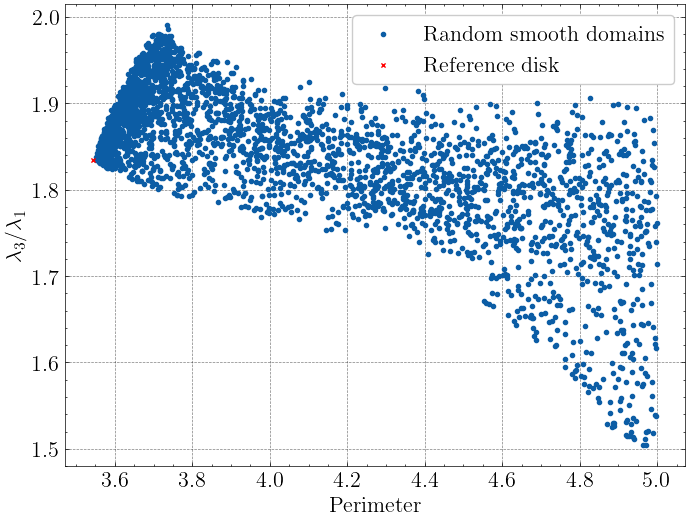
\includegraphics[width=\textwidth]{Images/Dirac/smooth/smooth_domains_scatter_benguria_third.png}
        \caption{Ratio between the third and first eigenvalues \(\frac{\lambda_3}{\lambda_1}\).}
        \label{dirac_smooth_domains_scatter_benguria_third}
    \end{minipage}
\end{figure}

Next, we investigate the domain with the smallest third eigenvalue, and we look for the minimizer of the functional
\begin{equation*}%\label{dirac_min_third_func}
    \mathcal{F}(\Omega) = \lambda_3(\Omega).
\end{equation*}

In general, one can address minimization problems in Banach spaces using the notion of \textit{Fréchet}-derivative. In shape optimization problems, for the eigenvalues of an elliptic operator one can use the variational formula for its eigenvalues. For example, the formula proved in Theorem \ref{spec_lap_pre} can be used to derive some results for the Laplacian Dirichlet problem. In fact, consider \(\Omega_t = \varphi(t)(\Omega)\) a small perturbation of \(\Omega\) in the parameter \(t\), where \(\varphi(t)\) is some diffeomorphism for small values of \(t\), 
\[
    \varphi(t) = I + t V
\]
for some fix vector field \(V\) and \(\Omega_0 = \Omega\). Let  \(\lambda_k(t)\) be an eigenvalue of the Laplace operator with Dirichlet boundary conditions on the domain \(\Omega_t\) and \(u^{(k)}_t\) its associated eigenfunction in \(H^1_0(\Omega_t)\). If \(\lambda_k\) has multiplicity one (if it is simple) and \(\Omega\) is of class \(C^2\) or convex, then
\[
    \lambda'_k(0) =- \int_{\partial\Omega} \left(\frac{\partial u^{(k)}_0}{\partial n}\right)^2 V\cdot n d \sigma.
\]
For more details, we point the reader to \cite{henrot2006extremum} and \cite{kato2013perturbation}.
As of the moment of writing, the author is not aware of any closed form for the derivative of the eigenvalues of the Dirac operator. In that case, two different strategies were considered to solve the unconstrained minimization problem
\begin{equation}\label{dirac_unconstrained_min_lambda_3}
    \min_{\substack{\Omega \subset \mathbb{R}^2 \\ \abs{\Omega}=1}} \mathcal{F}(\Omega).
\end{equation}

Starting from a given domain \(\Omega\), \(\mathcal{F}\) can be minimized using the Broyden–Fletcher–Goldfarb–Shanno (\ac{BFGS}) algorithm, a quasi-Newton method which uses the local curvature of \(\mathcal{F}\) to find the descent direction given by an approximation of the Hessian matrix. Unfortunately, the \ac{BFGS} method also needs the derivative at the point, which can only be numerically found using finite-difference methods. The second method is the multidimensional Nelder-Mead direct search method. Just like the bracketing algorithm used to find the singularities on the graph of the smallest singular value, the Nelder-Mead method does not use any information on the derivative and relies on evaluations of the loss function \(\mathcal{F}\) to bracket the local minima: in this case, a heuristic strategy with a multidimensional simplex is used to approximate it.

To apply both the \ac{BFGS} and the Nelder-Mead algorithms, one starts by approximate the domain \(\Omega_0\) with the lowest third eigenvalue by a polar parameterization. This is achieved by considering a sample of \(N\) boundary points from the domain, consider its polar coordinates and find the coefficients of a trigonometric interpolation. More precisely, let \(M\) be the order of the trigonometric interpolation. Assume that the radial part of each boundary point of \(\Omega_0\) can be parametrized by \(r(\theta)\), where \(\theta \in (0, 2\pi)\). In that case, one use the approximation
\[
    r(\theta_i) \approx a_0 + \sum_{m=1}^{M}a_m \cos(m \theta_i) + \sum_{m=1}^{M}b_m \sin(m \theta_i),
\]
where \(\theta_i\) is the polar part of the sample point \(i\) with \(i=1,\dots,N\). Then, the system
\[
    \begin{bmatrix}
        1 & \cos(1 x_1) & \cos(2 x_1) & \dots & \cos(M x_1) & \sin(1 x_1) & \dots & \sin(M x_1)\\
        \vdots & \vdots & \vdots & \vdots & \vdots & \vdots & \vdots & \vdots\\
        1 & \cos(1 x_N) & \cos(2 x_N) & \dots & \cos(M x_N) & \sin(1 x_N) & \dots & \sin(M x_N)
    \end{bmatrix}_{N\times(2M+1)}
    \begin{bmatrix}
        a_0\\
        \vdots\\
        b_M
    \end{bmatrix}
    =
    \begin{bmatrix}
        r(\theta_1)\\
        \vdots\\
        r(\theta_N)\\
    \end{bmatrix}
\]
can be solved by least squares when considering the over-determined system with \(N > 2M+1\). Notice that the problem \eqref{dirac_unconstrained_min_lambda_3} is now discretized into a finite-dimensional problem, since every domain is now a vector of coefficients in \(\mathbb{R}^{2M+1}\). Of course, one must still consider the domain generated by the found coefficients with unitary area.

In Figure \ref{dirac_nelder_mead_domain} it is presented an (almost) optimal domain \(\Omega^\star\) shape which minimizes the third eigenvalue of the Dirac operator with infinite-mass boundary conditions. This plot was obtained through the Nelder-Mead algorithm. The third eigenvalue of this domain is approximately \(\lambda_3 \approx 5.63787728\) and its perimeter \(L\) is \(L \approx 5.2650031\). In Figure \ref{dirac_val_third} we validate our findings by plotting the (continuous) family of one-parameter transformations (also known as a Minkowski sum) from the unit disk to \(\Omega^\star\), given by
\[
   \Omega_t = (1-t)\mathbb{D} + t \Omega^\star, \; 0 \leq t \leq 1.
\]
\begin{figure}[!htb]
    \centering
    \begin{minipage}{.5\textwidth}
        \centering
        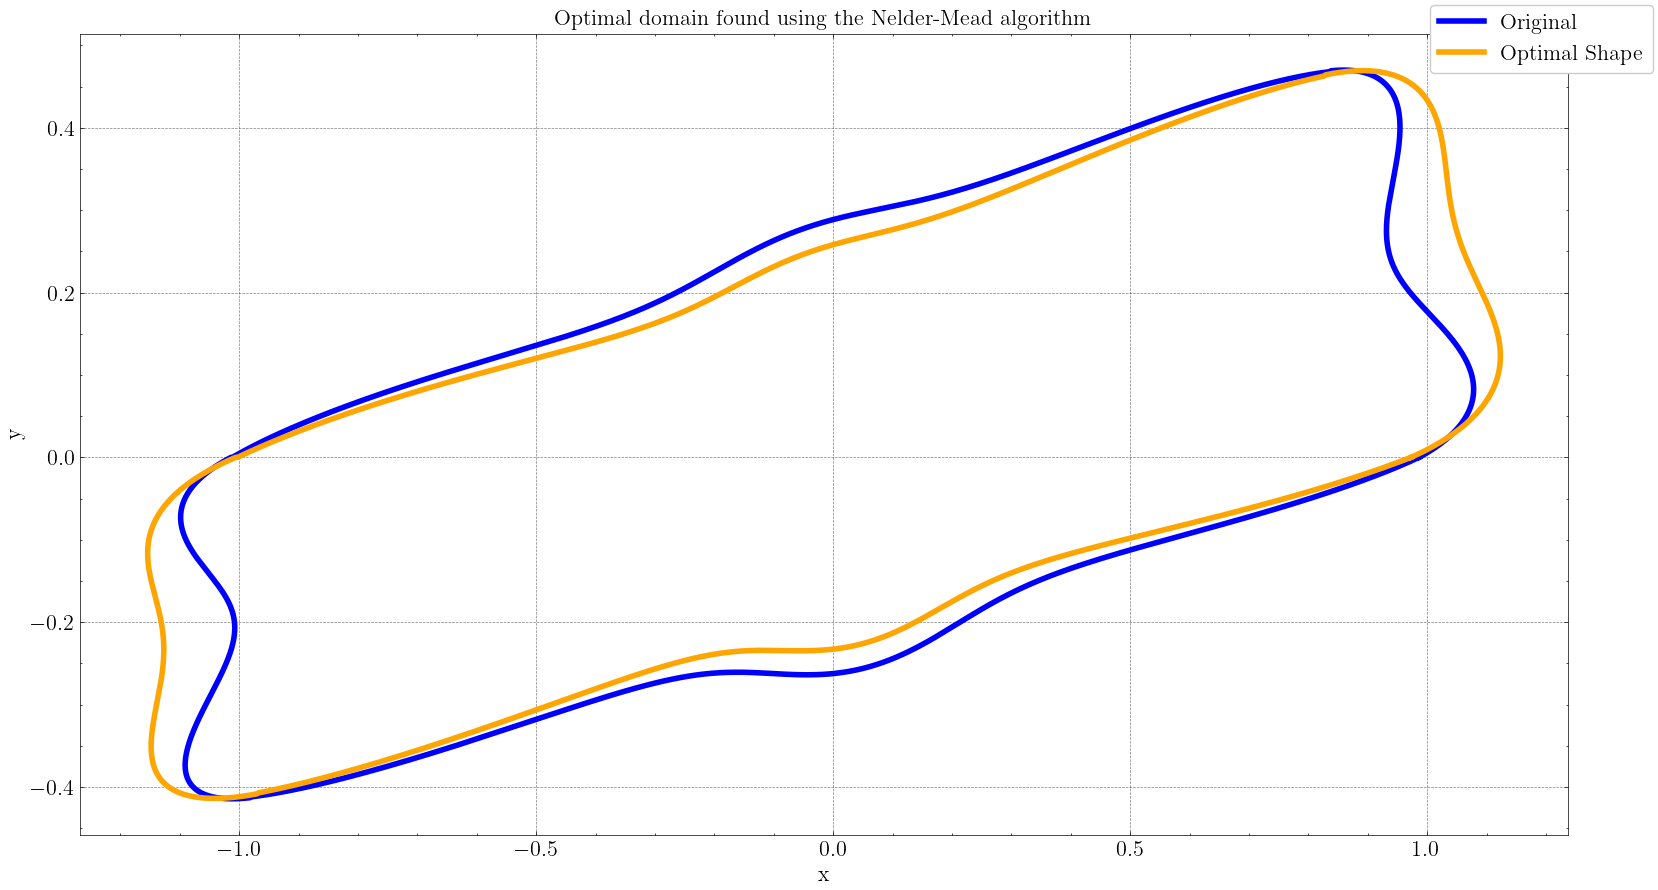
\includegraphics[width=1\linewidth]{Images/Dirac/smooth/nelder_mead_optimal.png}
        \captionsetup{width=0.8\linewidth} % Adjust the width of the caption
        \captionof{figure}{Optimal domain \(\Omega^\star\) (on orange) against the original domain in the first iteration of the Nelder-Mead algorithm.}
        \label{dirac_nelder_mead_domain}
    \end{minipage}%
    \hfill
    %\hspace{0.5cm} % Add some horizontal space between the figures
    \begin{minipage}{.5\textwidth}
        \centering
        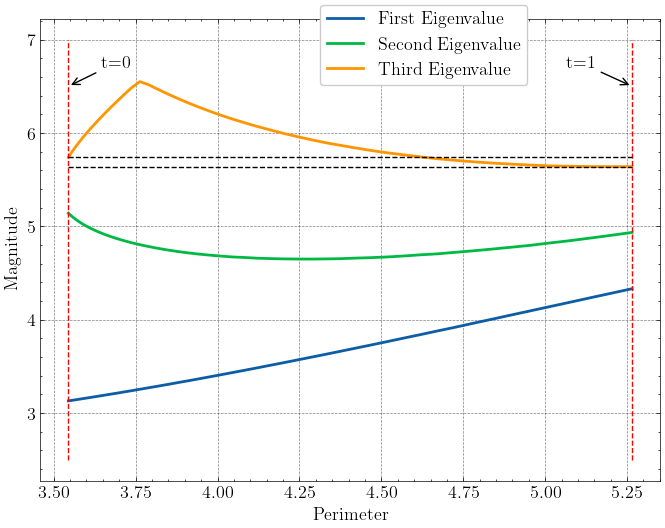
\includegraphics[width=0.9\linewidth]{Images/Dirac/smooth/dirac_val_third.png}
        \captionsetup{width=0.8\linewidth} % Adjust the width of the caption
        \captionof{figure}{Plot of the first three eigenvalues of the Minkowski sum \(\Omega_t\) for each increasing value of \(t\).}
        \label{dirac_val_third}
    \end{minipage}
\end{figure}

As said above, the \ac{BFGS} method was also used. However, no meaningful results were found using this method, since any descent direction produced not  

\begin{remark}
    One can not fail to point a valid criticism in this method: since we only parametrized the radial part of the domain's boundary, given the periodicity of the trigonometric interpolation one always end up with star-like shapes. Particularly, in our case, the order of the trigonometric interpolation was low, with \(M=4\). However, by increasing the order of interpolation the dimension of the optimization space would increase and, in this case, we are already working on \(\mathbb{R}^9\) and is very hard for a direct search method like Nelder-Mead to find a local minimum in such a ``high'' dimensional space. The option to only work with the radial part, instead of both cartesian components, was also a way to reduce the dimensionality of the problem. 
\end{remark}

Finally, the normalized eigenfunction associated with the optimal third eigenvalue of domain \(\Omega^\star\) are shown in Figure \ref{dirac_optimal_plots_eigenfunctions}.

\begin{figure}[!htb]
    \centering
    \begin{minipage}[b]{0.45\textwidth}
        \centering
        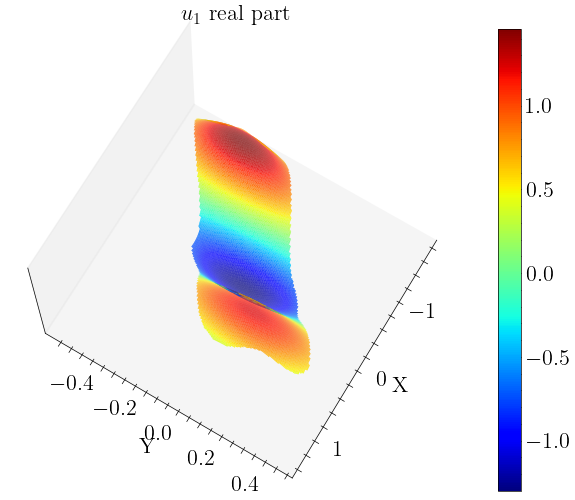
\includegraphics[width=0.8\textwidth]{Images/Dirac/smooth/optimal_lambda3_m_1_u1_re.png}
%\caption{Network 1}
    \end{minipage}
    \hfill
    \begin{minipage}[b]{0.45\textwidth}
        \centering
        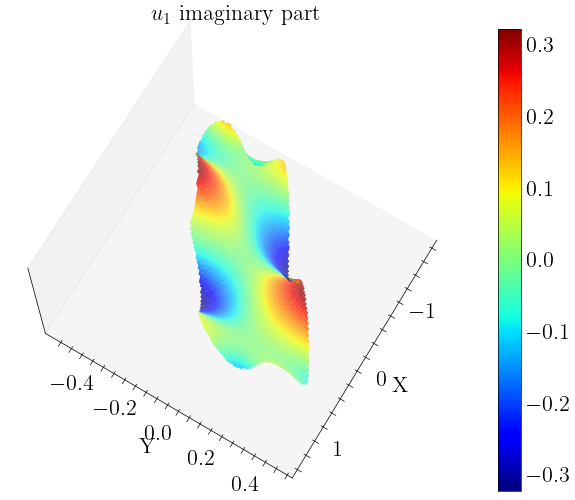
\includegraphics[width=0.8\textwidth]{Images/Dirac/smooth/optimal_lambda3_m_1_u1_im.png}
%\caption{Network 2}
    \end{minipage}

    \vspace{0.5cm}

    \begin{minipage}[b]{0.45\textwidth}
        \centering
        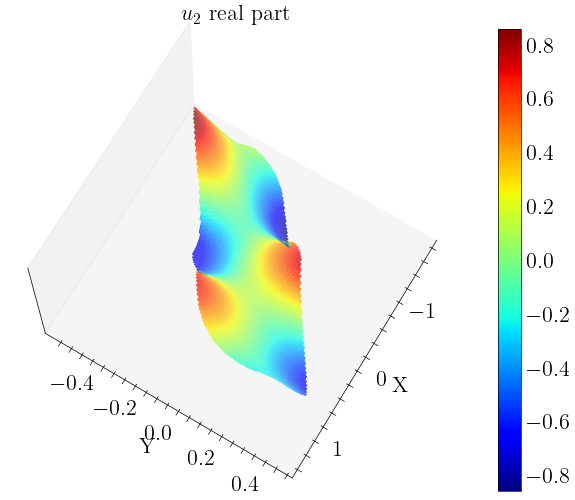
\includegraphics[width=0.8\textwidth]{Images/Dirac/smooth/optimal_lambda3_m_1_u2_re.png}
%\caption{Network 3}
    \end{minipage}
    \hfill
    \begin{minipage}[b]{0.45\textwidth}
        \centering
        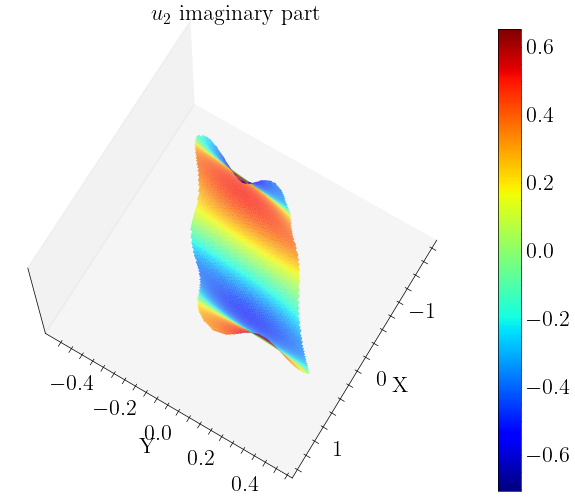
\includegraphics[width=0.8\textwidth]{Images/Dirac/smooth/optimal_lambda3_m_1_u2_im.png}
%\caption{Network 4}
    \end{minipage}
    \caption{Plots of the real and imaginary parts of \(u_1\) and \(u_2\) of the third eigenfunction \(\mathbf{u}=\begin{bmatrix} u_1\\ u_2 \end{bmatrix}\) associated with the optimal domain \(\Omega^\star\).}
    \label{dirac_optimal_plots_eigenfunctions}
\end{figure}

% \begin{figure}[!htb]
%     \centering
%     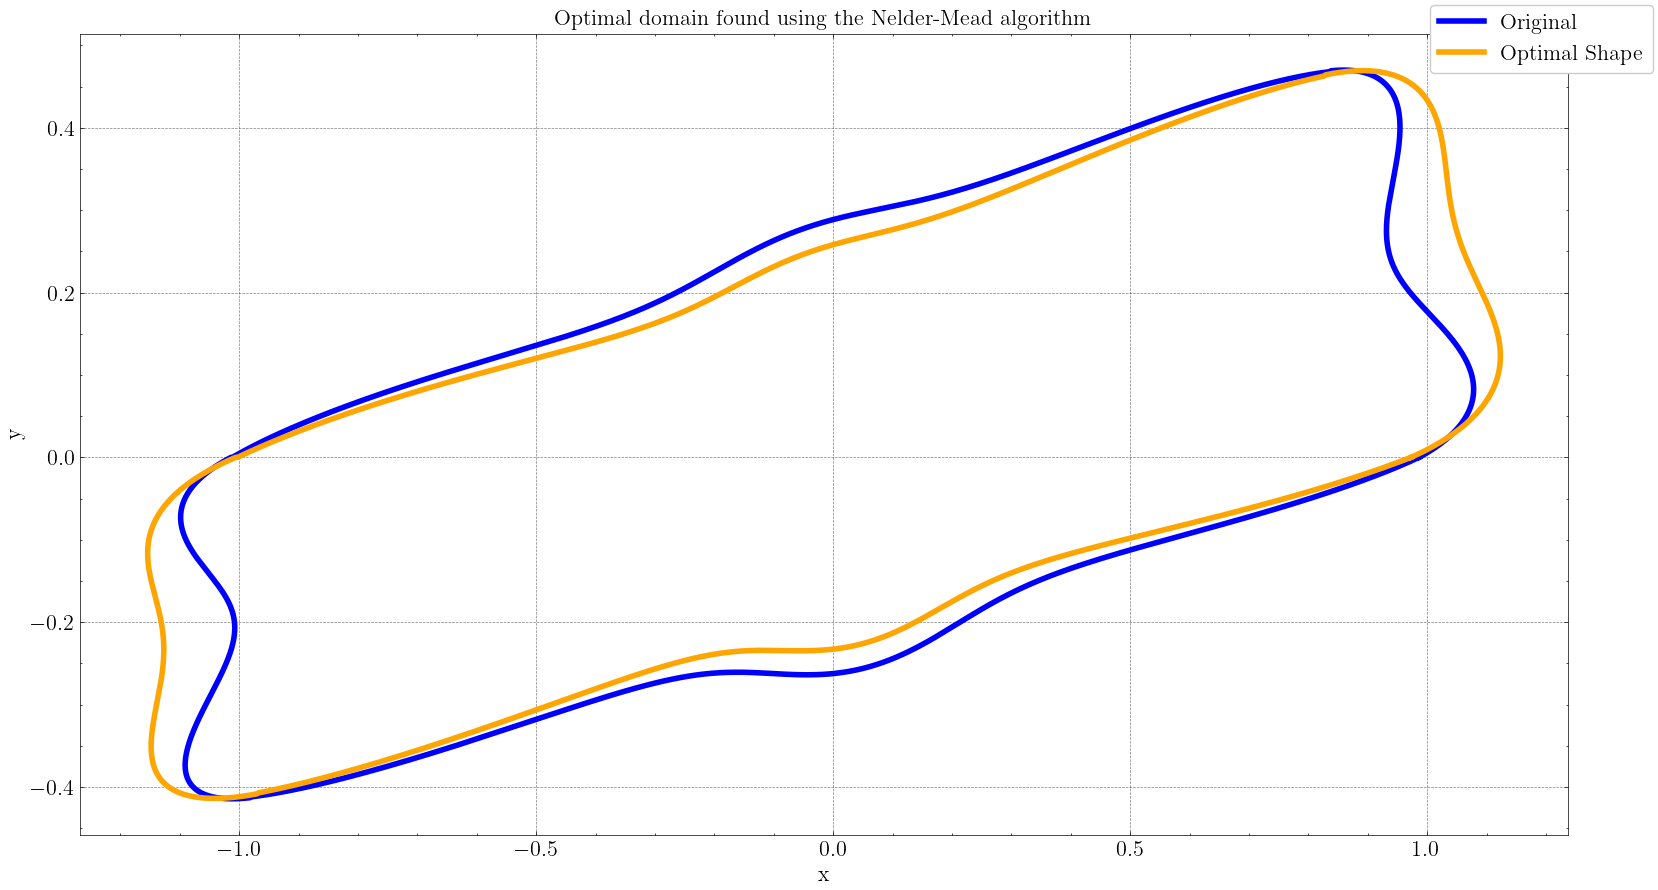
\includegraphics[width=0.75\linewidth]{Images/Dirac/smooth/nelder_mead_optimal.png}
%     \captionof{figure}{Some smooth domain generated by B-splines.}
%     \label{dirac_nelder_mead_domain}
% \end{figure}

% \begin{figure}[!htb]
%     \centering
%     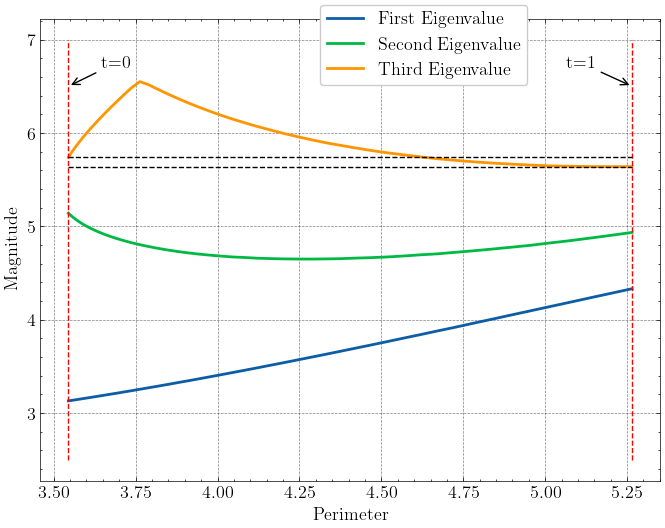
\includegraphics[width=0.75\linewidth]{Images/Dirac/smooth/dirac_val_third.png}
%     \captionof{figure}{Some smooth domain generated by B-splines.}
%     \label{dirac_val_third}
% \end{figure}

\section{Transmission problem simulations}\label{numerical_transmission_simulations}

For the Transmission problem, we now consider the set of equations studied previously in the subchapter \ref{domain_decomp_problem}, given by

\begin{align}\label{transmission_num}
    \begin{split}
    - \nabla k_i \nabla u_i &= f_i, \; \text{in }\Omega_i\\
    u_1 - u_2 &= 0, \; \text{on }\gamma\\
    k_1 \frac{\partial u_1}{\partial n_1} + k_2 \frac{\partial u_2}{\partial n_2} &= 0, \; \text{on }\gamma\\
    u_i &= 0, \; \text{on }\Gamma_i.
    \end{split}
\end{align}

Like before, the domain \(\Omega \subset \mathbb{R}^2\) is divided into two non-overlapping regions \(\Omega_1\) and \(\Omega_2\) such that \(\overline{\Omega} = \overline{\Omega_1} \cup \overline{\Omega_2}\). Their common boundary is denoted by \(\gamma = \partial\Omega_1 \cap \partial\Omega_2\) and the boundary of each domain (minus the common boundary) is also denoted by \(\Gamma_i = \partial\Omega_1\setminus{\gamma}\). In what follows, the source functions \(f_i\) of each domain are constant\footnote{In this work we only considered \(f_i=1\). In any case, we are still working with a general discontinuous source function (if \(k_1 \neq k_2\)). Working with different \textit{continuous} source functions should make no difference in the result. We will also present how to deal with general and continuous source functions.}, and we took \(f_i = 1\). Recall that \(k_1 \geq k_2 > 0\) are constants and \(n_i\) is the (normalized) outward normal to each domain subdomain \(\Omega_i, i=1, 2\), where we shall write \(n=n_1=-n_2\) when we are restricted to the interface.

The procedure presented here is based on \cite{alves2005new} and \cite{alves2021domain}. Given that \(f_i = 1\) for each \(i=1, 2\), a solution of \eqref{transmission_num} can be found by taking the following steps:
\begin{enumerate}
    \item Find a solution for the non-homogeneous problem
    \[
        \begin{cases}
            -\Delta u_1^{NH} = \frac{1}{k_1}\\
            -\Delta u_2^{NH} = \frac{1}{k_2}.
        \end{cases}
    \]
    This can easily be done, and we have
    \[
        \begin{cases}
            u_1^{NH} = -\frac{x_1^2 + x_2^2}{4k_1}\\
            u_2^{NH} = -\frac{x_1^2 + x_2^2}{4k_2};
        \end{cases}
    \]
    \item Then we solve the homogeneous problem
    \begin{align}\label{transmission_num_homo}
        \begin{split}
        - \Delta u_i^H &= 0, \; \text{in }\Omega_i\\
        u_1^H - u_2^H &= u_2^{NH}- u_1^{NH}, \; \text{on }\gamma\\
        k_1 \frac{\partial u_1}{\partial n_1} - k_2 \frac{\partial u_2}{\partial n_1} &= k_2 \frac{\partial u_2^{NH}}{\partial n_1}  - k_1 \frac{\partial u_1^{NH}}{\partial n_1}, \; \text{on }\gamma\\
        u_i &= - u_i^{NH}, \; \text{on }\Gamma_i;
        \end{split}
    \end{align}
    \item Finally, the solution of \eqref{transmission_num} is \(u_i = u_i^H + u_i^{NH}\).
\end{enumerate}
For general source functions, the steps above can also be used: however, it may not be possible to find an analytical solution in first step. In this case, \textbf{1.} must be solved numerically. A popular choice is to use radial basis functions (\ac{RBF}s) (see \cite{golberg1996improved} for example), like the thin plate spline
\[
    \varphi(r) = r^2 \log r,     
\]
and find the coefficients \(\alpha_j\) in \(f_i(x_k) = \tilde{f}_i(x_k) = \sum_{j=1}^{n} \alpha_j \varphi_j(x_k)\) using least square methods, where \(x_k\) are collocation points. Finally, one can analytically solve the equation \(-\Delta \Psi_j = \varphi_j\) to recover the non-homogeneous solutions \(u_1^{NH}\) and \(u_2^{NH}\). In \cite{alves2005new} and \cite{alves2021domain} a different approach was suggested using the fundamental solutions of the Helmholtz equation instead of the classical \ac{RBF}s; that method is known today as \textit{Kansa MFS method}.

In what follows, the numerical results illustrate the accuracy of the method in simply connected 2D domains. Let \(N_i\) denote the number of source points for each domain \(i\), such that \(N=N_1+N_2\). We denote the approximate solution by
\[
    \tilde{u} = \begin{cases}
        \tilde{u}_1, & \text{in } \Omega_1\\
        \tilde{u}_2, & \text{in } \Omega_2,
    \end{cases}
\]
where
\begin{align*}
    &\tilde{u}_1(x) = \sum_{j=1}^{N_1} \alpha^{(1)}_j \Phi\left(x-y_j^{(1)}\right)\\
    &\tilde{u}_2(x) = \sum_{j=1}^{N_2} \alpha^{(2)}_j \Phi\left(x-y_j^{(1)}\right).
\end{align*}
Let \(M_i\) be the number of boundary collocation points \(x^{(i)}_{m}\) for each \(\Omega_i\) and \(M=M_1+M_2\). We also consider \(Q\) interface points \(z_q \in \gamma\) with \(q=1,\dots,Q\). Then, a full block system is written as
\begin{equation}\label{mfs_transmission_classical_matrices_system}
    \renewcommand{\arraystretch}{1.75} % Increase spacing between rows of the matrices
    \begin{bmatrix}
        \left[\Phi\left(x^{(1)}_{m}-y_j^{(1)}\right)\right] & [0] \\
        [0] & \left[\Phi\left(x^{(2)}_{m}-y_j^{(2)}\right)\right] \\
        \left[\Phi\left(z_q-y_j^{(1)}\right)\right] & \left[-\Phi\left(z_q-y_j^{(2)}\right)\right] \\
        \left[k_1\partial_n \Phi\left(z_q-y_j^{(1)}\right)\right] & \left[-k_2 \partial_n \Phi\left(z_q-y_j^{(2)}\right)\right]
    \end{bmatrix}
    \begin{bmatrix}
        \left[\alpha^{(1)}_j\right]\\
        \left[\alpha^{(2)}_j\right]
    \end{bmatrix}=
    \begin{bmatrix}
        \left[-u_1^{NH}(x^{(1)}_{m})\right]\\
        \left[-u_2^{NH}(x^{(2)}_{m})\right]\\
        \left[u_2^{NH}(z_q)-u_1^{NH}(z_q)\right]\\
        \left[k_2 \partial_n u_2^{NH}(z_q)- k_1 \partial_n u_1^{NH}(z_q)\right]\\
    \end{bmatrix}
\end{equation}

Most of the examples below do not have analytical solution: only in the subsection \ref{transmission_val_subsection}, when we test the results against a known solution, we are able to find the absolute error. In the other cases we are only interested in the relative error, i.e, the boundary error (against which we can compare since \(u_i=0\) in \(\Gamma_i\)) and the interface error by checking the transmission conditions on \(\gamma\):
\begin{itemize}
    \item \(\norm*{\tilde{u}_i - 0}_{L^2(\Gamma_i)}\), \(i=1, 2\): boundary collocation error;
    \item \(\norm*{\tilde{u}_1 - \tilde{u}_2}_{L^2(\gamma)}\), \(i=1, 2\): continuity error (\(C^0\)) of \(\tilde{u}\) across \(\gamma\);
    \item \(\norm*{k_1 \partial_n\tilde{u}_1 - k_2 \partial_n\tilde{u}_2}_{L^2(\gamma)}\), \(i=1, 2\): continuity error \(C^1\) of \(\partial_n\tilde{u}\) across \(\gamma\).
\end{itemize}
From a numerical point of view, let \(\mathcal{I}\) be the sample of test points. The \(L^2\) norm is discretized into the Root Mean Squared Error (\ac{RMSE}) which is equivalent to the \(l^2\) norm and is given by
\[
    \norm*{u-\tilde{u}}= \sqrt{\frac{1}{\#\mathcal{I}} \sum_{z \in \mathcal{I}} \abs{u(z)-\tilde{u}(z)}^2}.
\]
For every result below the number of sample test points is 5 times larger than the sample used to find the coefficients of the MFS, and we fix \(k_2=1\) since the ratio \(\frac{k_1}{k_2}\) is responsible for the behavior of the solutions near the interface. 

\subsection{Numerical validation of the method}\label{transmission_val_subsection}

First, we start by testing the numerical algorithm for the unit disk \(\mathbb{D}\), with \(k_1=k_2=1\). From Theorem \eqref{equivalence_transmission}, we know that the system of differential equations \eqref{transmission_num} is equivalent to the Poisson equation
\begin{align}\label{transmission_disk}
    \begin{split}
        -\Delta u = 1, & \text{ in } \mathbb{D}\\
        u = 0, & \text{ on } \partial\mathbb{D},
    \end{split}
\end{align}
and is easy so see that the exact solution of Equation \eqref{transmission_disk} is given in polar coordinates by \(u(r, \theta) = \frac{1-r^2}{4}\). 

\begin{figure}[!htb]
    \centering
    \begin{minipage}{.5\textwidth}
      \centering
      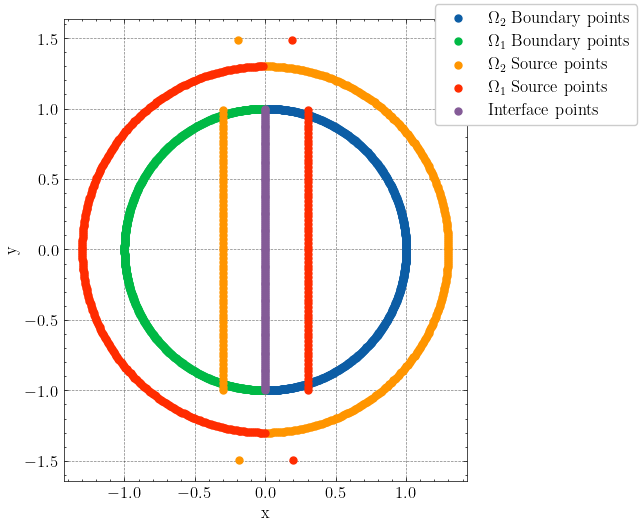
\includegraphics[width=1\linewidth]{Images/Transmission/Circle_val_col_points_600_150.png}
      \captionsetup{width=0.9\linewidth} % Adjust the width of the caption
      \captionof{figure}{Configuration of the boundary, source and interface points. Each domain has 600 boundary points, 377 source points and the common interface has 100 points.}
      \label{transmission_disk_col}
    \end{minipage}%
    %\hspace{0.5cm} % Add some horizontal space between the figures
    \begin{minipage}{.5\textwidth}
      \centering
      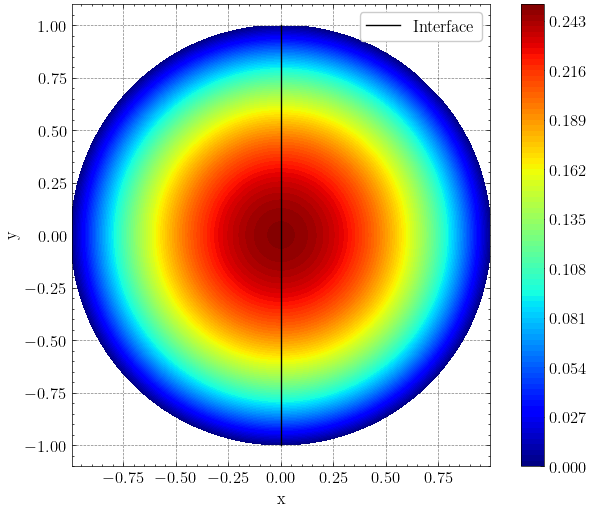
\includegraphics[width=1\linewidth]{Images/Transmission/Circle_val_contour_600_150.png}
      \captionsetup{width=0.9\linewidth} % Adjust the width of the caption
      \captionof{figure}{Numerical approximation of the \ac{BVP} \eqref{transmission_disk} under the conditions presented in Figure \ref{transmission_disk_col}}
      \label{transmission_disk_plot}
    \end{minipage}
\end{figure}

The absolute error between the approximate solution and the exact solution can then be calculated for each domain point. The sample points to compute the absolute error were generated in a uniform grid and were also used to plot Figure \ref{transmission_disk_plot}. The method described at the end of the subchapter \ref{density_proofs_section} was used to place the source points, where \(\eta=0.3\).

\begin{table}[htbp]
    \centering
    \begin{tabular}{cccccc}
        \toprule
        \multirow{2}{*}{\textbf{Boundary/Interface Points}} & \multicolumn{2}{c}{\textbf{Boundary Error}} & \multicolumn{2}{c}{\textbf{Absolute Error}} \\
        \cmidrule(lr){2-3} \cmidrule(lr){4-5}
        & \textbf{Domain 1} & \textbf{Domain 2} & \textbf{Domain 1} & \textbf{Domain 2} \\
        \midrule
        600/150 & $9.759\times10^{-12}$ & $9.541\times10^{-12}$ & $1.465\times10^{-11}$ & $1.439\times10^{-11}$ \\
        500/100 & $3.667\times10^{-11}$ & $3.945\times10^{-11}$ & $9.382\times10^{-11}$ & $9.310\times10^{-11}$ \\
        412/100 & $3.721\times10^{-11}$ & $5.036\times10^{-11}$ & $9.652\times10^{-11}$ & $9.584\times10^{-11}$ \\
        \bottomrule
    \end{tabular}
    \caption{Numerical errors for the boundary and the whole Domains \(\Omega_1\) and \(\Omega_2\)}
    \label{tab:transmission_results_1}
\end{table}


\begin{table}[htbp]
    \centering
    \begin{tabular}{cccc}
      \toprule
      \textbf{Boundary/Interface Points} & \textbf{Interface \(C^0\) Error} & \textbf{Interface \(C^1\) Error} & \textbf{Condition number} \\
      \midrule
      600/150 & $6.945\times10^{-11}$ & $1.841\times10^{-11}$ & $2.528\times 10^{19}$\\
      500/100 & $3.910\times10^{-10}$ & $1.100\times10^{-10}$ & $2.382\times 10^{18}$\\
      412/100 & $4.035\times10^{-10}$ & $1.342\times10^{-10}$ & $7.597\times 10^{17}$\\
      \bottomrule
    \end{tabular}
    \caption{Numerical error on the interface \(\gamma\). The condition number of the matrix is also presented.}
    \label{tab:transmission_results_2}
\end{table}

The numerical results presented in Tables \ref{tab:transmission_results_1} and \ref{tab:transmission_results_2} are not yet optimal. When considering a larger value of \(\eta\), the results increase by more than two orders of magnitude, but this also leads to a significant increase in the already very high condition number (see Table \ref{tab:transmission_results_2}), as expected. Despite this, the results show great promise, which was anticipated due to the domain's analyticity.

As mentioned previously, the Method of Fundamental Solutions (MFS) yields better results in highly regular domains, even when considering curved geometries. However, increasing the number of boundary and interface collocation points improves the accuracy of the solution. It is important to note that a larger number of points also escalates the condition number, making the problem more challenging to solve accurately.

The inclusion of the "corner" source points, as depicted in Figure \ref{transmission_disk_col}, also significantly impacts the method's accuracy. These source points, strategically added to capture the behavior near the interface corner, can be inside one of the domains as the solution will be split into two parts.

\subsection{Results for the rectangle}

In this subsection a rectangular domain \([-1, -0.5] \times [1, 0.5]\) with a vertical interface along the line \(x=0\) is considered. We are now interested to study the problem for \(k_1 \neq k_2\) where \(k_2=1\) is fixed. The results below were conducted with 600 boundary points and 404 source points for each domain. The number of interface points is 150 and \(\eta=0.08\).

\begin{figure}[!htb]
    \centering
    \begin{minipage}{.5\textwidth}
      \centering
      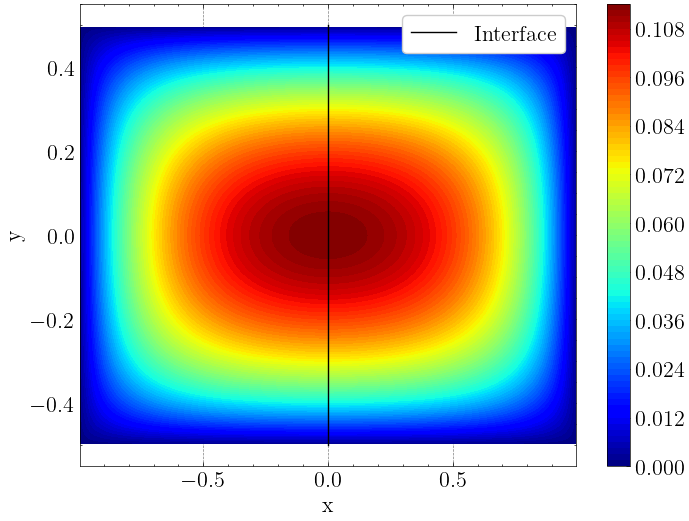
\includegraphics[width=\linewidth]{Images/Transmission/Rectangle_contour_600_150_k1_1.png}
      \caption{Numerical simulation with  \(k_1=1\).}
      \label{transmission_rectangle_plot_k1_1}
    \end{minipage}%
    \begin{minipage}{.5\textwidth}
      \centering
      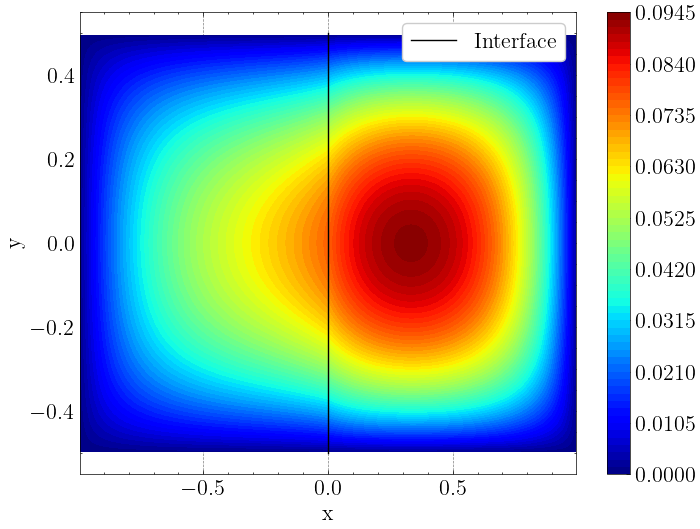
\includegraphics[width=\linewidth]{Images/Transmission/Rectangle_contour_600_150_k1_2.png}
      \caption{Numerical simulation with \(k_1=2\).}
      \label{transmission_rectangle_plot_k1_2}
    \end{minipage}
    
    \vspace{0.5cm} % Add some vertical space between the rows of figures
    
    \begin{minipage}{.6\textwidth}
      \centering
      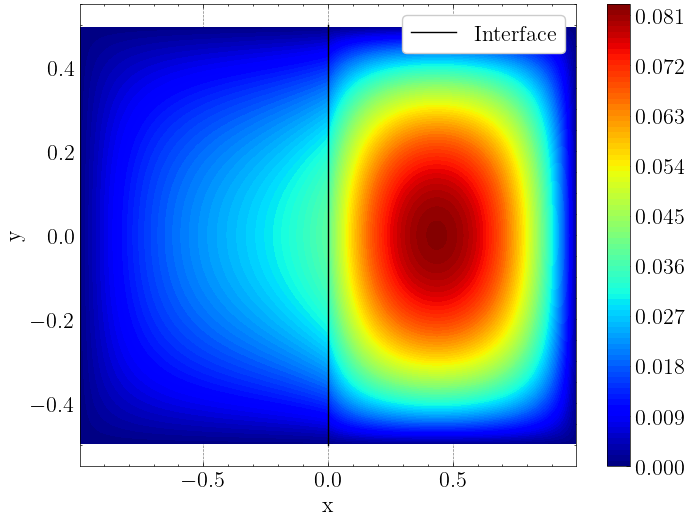
\includegraphics[width=0.9\linewidth]{Images/Transmission/Rectangle_contour_600_150_k1_5.png}
      \caption{Numerical simulation with  \(k_1=5\).}
      \label{transmission_rectangle_plot_k1_5}
    \end{minipage}
    
    \caption*{Numerical approximations of the \ac{BVP} for a rectangular domain with different \(k_1\) values.}
    \label{transmission_rectangle_plots}
\end{figure}

\begin{table}[htbp]
    \centering
    \begin{tabular}{cccccc}
      \toprule
      \multirow{2}{*}{\textbf{\(k_1\) value}} & \multicolumn{2}{c}{\textbf{Boundary Error}} & \multicolumn{2}{c}{\textbf{Interface Errors}} & \multirow{2}{*}{\textbf{Condition number}} \\
      \cmidrule(lr){2-3} \cmidrule(lr){4-5}
      & \textbf{Domain 1} & \textbf{Domain 2} & \textbf{\(C^0\)} & \textbf{\(C^1\)} & \\
      \midrule
      1 & $7.775\times10^{-8}$ & $7.779\times10^{-8}$ & $4.732\times10^{-9}$ & $7.589\times10^{-9}$ & $2.331\times 10^{13}$\\
      2 & $4.398\times10^{-8}$ & $8.614\times10^{-8}$ & $2.499\times10^{-6}$ & $7.868\times10^{-8}$ & $3.623\times 10^{13}$\\
      3 & $2.181\times10^{-8}$ & $1.036\times10^{-7}$ & $3.838\times10^{-6}$ & $1.551\times10^{-7}$ & $8.182\times 10^{13}$\\
      \bottomrule
    \end{tabular}
    \caption{Numerical relative error on the boundary and in the interface \(\gamma\)}
    \label{tab:transmission_results_rectangle}
\end{table}

In Figures \ref{transmission_rectangle_plot_k1_1}, \ref{transmission_rectangle_plot_k1_2}, and \ref{transmission_rectangle_plot_k1_5}, we present the numerical approximation for different \(k_1\) values. Observe that increasing \(k_1\) breaks the symmetry of the solution, which shifts from \(\Omega_1\) (the domain on the left) to \(\Omega_2\) (the domain on the right). Table \ref{tab:transmission_results_rectangle} summarizes the results for different \(k_1\) values. While the results are slightly worse than the previous ones due to the worse domain regularity, they still preserve high accuracy. It is worth noting that for different values of \(k_1\) and \(k_2\), the accuracy of the method decreases. This is also to be expected, as we are dealing with a discontinuous source function, which decreases the regularity of the solution.

Notice that the condition number for the rectangle is smaller than the one presented in Table \ref{tab:transmission_results_2} for the unit disk. This is a consequence of a smaller value of \(\eta\), which in this case appears to be optimal, since increasing its value decreases the overall accuracy.

\subsection{Results for an L-shape domain with enrichment}

In the previous subsection, a domain with corners was analyzed. However, it still preserved some regularity, and the MFS with classical basis functions was able to capture its corner's behavior, as explained in Remark \ref{particular_solutions}. In what follows, we are going to study the case of an L-shape, a non-convex domain with singular corners. Two different interfaces will be considered: first, the usual interface along the line \(x=0\); then, along its symmetry axis with the line \(y=\frac{1}{2}x\).

Consider the L-shape given in Figure \ref{transmission_L_shape_config}. The left and right subdomains are denoted by \(\Omega_1\) and \(\Omega_2\), respectively. The number of interface points is 300, and the number of source points for each domain is 428. The number of boundary collocation points for \(\Omega_1\) and \(\Omega_2\) is 710 and 639, respectively.


% \begin{figure}[!htb]
%         \centering
%         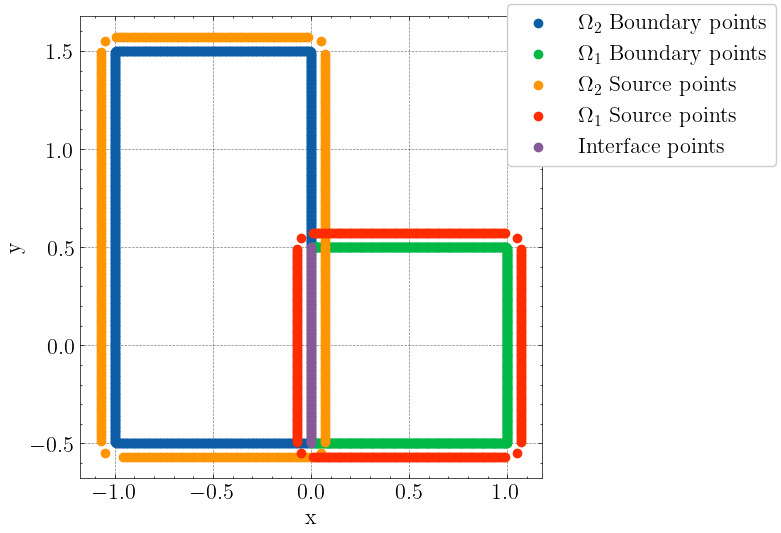
\includegraphics[width=0.5\linewidth]{Images/Transmission/L_shape_2_rectangles_col_points.png}
%         \caption{L-shape domain with vertical interface. Configuration of the boundary, source and interface points.}
%         \label{transmission_L_shape_config}
% \end{figure}

\begin{figure}[!htb]
    \centering
    \begin{minipage}{.5\textwidth}
        \centering
        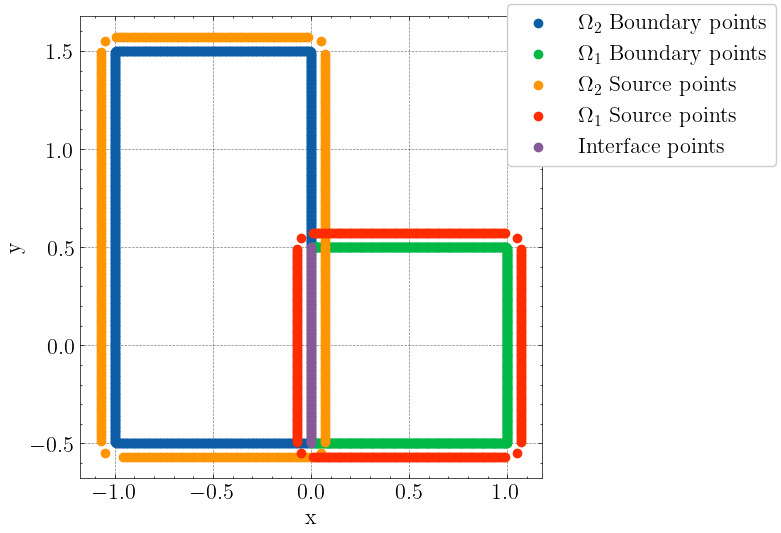
\includegraphics[width=0.8\linewidth]{Images/Transmission/L_shape_2_rectangles_col_points.png}
        \captionsetup{width=0.9\linewidth} % Adjust the width of the caption
        \caption{L-shape domain with vertical interface. Configuration of the boundary, source and interface points.}
        \label{transmission_L_shape_config}
    \end{minipage}%
    %\hspace{0.2cm} % Add some horizontal space between the figures
    \begin{minipage}{.5\textwidth}
        \centering
        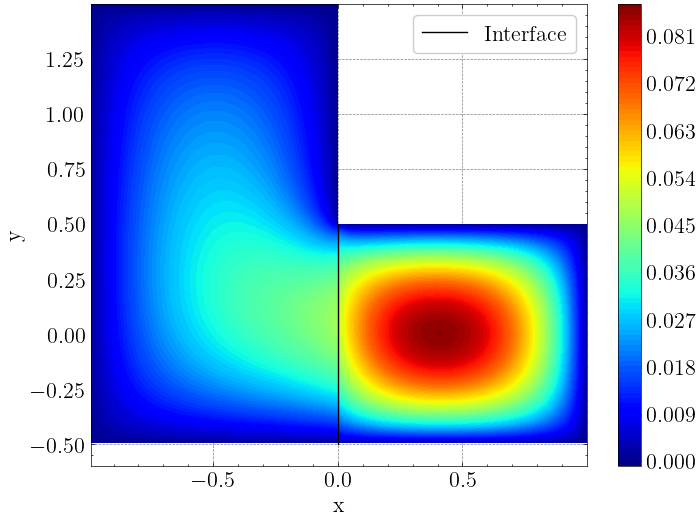
\includegraphics[width=\linewidth]{Images/Transmission/L_shape_2_rectangles_k1_5.png}
        \captionsetup{width=0.9\linewidth} % Adjust the width of the caption
        \caption{Numerical approximation of the \ac{BVP} for an L-shape domain with interface along \(x=0\) and \(k_1=5\).}
        \label{transmission_L_shape_k1_5}
    \end{minipage}
\end{figure}

In Table \ref{tab:transmission_results_L_shape_rectangles}, the results without resorting to enrichment are presented. It is evident that the method yields poorer results due to the lower regularity of the domain. Particularly, the interface error (mainly the \(C^0\) error) is significantly higher compared to previous cases, even when considering more collocation points on the interface. In fact, it appears that the domain itself poses more challenges than the discontinuous source function when considering different values for \(k_1\) and \(k_2\). In Figure \ref{transmission_L_shape_k1_5}, it is even possible to see that there already exists some small jump near the edges of the interface.

\begin{table}[htbp]
    \centering
    \begin{tabular}{cccccc}
      \toprule
      \multirow{2}{*}{\textbf{\(k_1\) value}} & \multicolumn{2}{c}{\textbf{Boundary Error}} & \multicolumn{2}{c}{\textbf{Interface Errors}} & \multirow{2}{*}{\textbf{Condition number}} \\
      \cmidrule(lr){2-3} \cmidrule(lr){4-5}
      & \textbf{Domain 1} & \textbf{Domain 2} & \textbf{\(C^0\)} & \textbf{\(C^1\)} & \\
      \midrule
      1 & $7.853\times10^{-5}$ & $1.155\times10^{-4}$ & $2.916\times10^{-3}$ & $2.155\times10^{-5}$ & $5.587\times 10^{12}$ \\
      2 & $8.152\times10^{-5}$ & $1.350\times10^{-4}$ & $3.835\times10^{-3}$ & $1.149\times10^{-5}$ & $8.161\times 10^{12}$ \\
      5 & $7.079\times10^{-5}$ & $1.378\times10^{-4}$ & $4.085\times10^{-3}$ & $5.411\times10^{-5}$ & $1.776\times 10^{13}$ \\
      \bottomrule
    \end{tabular}
    \caption{Numerical relative error on the boundary and in the interface \(\gamma\)}
    \label{tab:transmission_results_L_shape_rectangles}
\end{table}


One of the major problems for the method is the behavior of the solution near the degenerate corner with \(\pi\) radians in \(\Omega_1\), where some singularity may exist due to the different boundary conditions imposed there. Notice that for \(\Omega_2\) there exists no problem since the interface edges makes a right angle with the adjacent edges. Therefore, we consider some particular solutions which describe the solution in the domain \(\Omega_1\). In this case, we are going to use Dirichlet-Neummann particular solutions, like the ones presented in \ref{m_particular_solutions}, centered in the singular corner. Let
\begin{equation}\label{pat_sol_L_shape_rect}
    v_{p_1}(r, \theta) = \alpha_{p_1} r^{\alpha_{p_1}} \sin(\alpha_{p_1}(\theta - \theta_1))
\end{equation}
where
\[
    \alpha_{p_1} = \frac{(p+\frac{1}{2})\pi}{\Theta},
\]
\(\theta_1 = \frac{\pi}{2}\) is the angle shift, \(\Theta = \pi\) is the total angle amplitude,  and the coordinates \(r\) and \(\theta\) are given in polar coordinates by
\[
    r(x,y) = \sqrt{x^2+y^2} \quad \theta(x,y)=\begin{cases}
        \arctan(\frac{y}{x}),& \text{if} \arctan(\frac{y}{x})>0\\
        \arctan(\frac{y}{x})+2\pi,& \text{if} \arctan(\frac{y}{x})\leq0.
    \end{cases}
\]
By differentiating Equation \eqref{pat_sol_L_shape_rect} in cartesian coordinates and substituting polar coordinates again we find that
\begin{equation*}
    \nabla v_{p_1}(r, \theta) = \left(-\frac{(2 \pi  {p_1}+\pi )^2 r^{\frac{2 \pi  {p_1}+\pi }{2 \Theta }} \sin \left(\theta +\frac{\pi  \left(p_1+\frac{1}{2}\right) (s-\theta )}{\Theta }\right)}{4 \Theta ^2 r},\frac{(2 \pi  p_1+\pi )^2 r^{\frac{2 \pi  p_1+\pi }{2 \Theta }} \cos \left(\theta +\frac{\pi  \left(p_1+\frac{1}{2}\right) (s-\theta )}{\Theta }\right)}{4 \Theta ^2 r}\right).
\end{equation*}
Finally, considering the truncated expansion
\begin{equation}\label{num_particular_L_shape_rect_equation}
    \phi(r,\theta)=\sum_{p_1=0}^{P_1} \beta_{p_1} v_{p_1}(r, \theta),
\end{equation}
and expanding the matrix in \eqref{mfs_transmission_classical_matrices_system}, one can write
\begin{equation}\label{transmission_mat_L_rect_exp}
    \renewcommand{\arraystretch}{1.75} % Increase spacing between rows of the matrices
    \begin{bmatrix}
        \left[\Phi\left(x^{(1)}_{m}-y_j^{(1)}\right)\right] & [0] & \left[\phi(r\left(x_m\right),\theta\left(x_m\right))\right]\\
        [0] & \left[\Phi\left(x^{(2)}_{m}-y_j^{(2)}\right)\right] & \left[0\right]\\
        \left[\Phi\left(z_q-y_j^{(1)}\right)\right] & \left[-\Phi\left(z_q-y_j^{(2)}\right)\right] & \left[\phi(r\left(z_k\right),\theta\left(z_q\right))\right]\\
        \left[k_1\partial_n \Phi\left(z_q-y_j^{(1)}\right)\right] & \left[-k_2 \partial_n \Phi\left(z_q-y_j^{(2)}\right)\right] & \left[k_1 \partial_n\phi(r\left(z_q\right),\theta\left(z_q\right))\right]
    \end{bmatrix}
\end{equation}

Table \ref{tab:transmission_results_L_shape_rectangles_particular} presents the results after applying the enrichment technique for the previous \(k_1\) values. In the expansion \eqref{num_particular_L_shape_rect_equation}, different values for \(P_1\) were considered. For example, for the first section of the Table, we set \(P_1=1\). After some simulations, it became clear that increasing \(P_1\) would not give better results. Furthermore, since the form of Equation \eqref{num_particular_L_shape_rect_equation} is also valid for the exterior problem, negative values of \(p_1\) were considered. Interestingly, when adding solutions for the exterior problem, better results were achieved. Not only did the error decrease for the boundary \(\Gamma_i\) of each domain, but better results were also achieved on the interface.

\begin{table}[htbp]
    \centering
    \begin{longtable}{ccccccc}
        \toprule
        \multicolumn{1}{c}{\textbf{\(p_1\) values}} & \multicolumn{1}{c}{\textbf{\(k_1\) value}} & \multicolumn{2}{c}{\textbf{Boundary Error}} & \multicolumn{2}{c}{\textbf{Interface Errors}} & \multicolumn{1}{c}{\textbf{Condition number}} \\
        \cmidrule(lr){2-2} \cmidrule(lr){3-4} \cmidrule(lr){5-6} \cmidrule(lr){7-7}
        & & \textbf{Domain 1} & \textbf{Domain 2} & \textbf{\(C^0\)} & \textbf{\(C^1\)} & \\
        \midrule
        \endfirsthead % Header for the first page
        \multicolumn{7}{l}{{\footnotesize\emph{Continued from previous page}}} \\
        \toprule
        \multicolumn{1}{c}{\textbf{\(p\) value}} & \multicolumn{1}{c}{\textbf{\(k_1\) value}} & \multicolumn{2}{c}{\textbf{Boundary Error}} & \multicolumn{2}{c}{\textbf{Interface Errors}} & \multicolumn{1}{c}{\textbf{Condition number}} \\
        \cmidrule(lr){2-2} \cmidrule(lr){3-4} \cmidrule(lr){5-6} \cmidrule(lr){7-7}
        & & \textbf{Domain 1} & \textbf{Domain 2} & \textbf{\(C^0\)} & \textbf{\(C^1\)} & \\
        \midrule
        \endhead % Header for subsequent pages
        \midrule[\heavyrulewidth] % Horizontal line
        \multicolumn{7}{r}{{\footnotesize\emph{Continued on next page}}} \\
        \endfoot % Footer for subsequent pages
        \bottomrule
        \endlastfoot % Footer for the last page
        
        % Data for p = [0, 1]
        0, 1 & 1 & $2.965\times10^{-5}$ & $7.907\times10^{-5}$ & $2.94\times10^{-3}$ & $2.624\times10^{-5}$ & $5.584\times10^{12}$ \\
        & 2 & $2.203\times10^{-5}$ & $6.657\times10^{-5}$ & $1.86\times10^{-3}$ & $2.068\times10^{-5}$ & $8.156\times10^{12}$ \\
        & 5 & $2.203\times10^{-5}$ & $6.657\times10^{-5}$ & $1.86\times10^{-3}$ & $2.068\times10^{-5}$ & $8.156\times10^{12}$ \\
        \midrule[\heavyrulewidth] % Horizontal line
        
        % Data for p = [-1, 0, 1]
        -1, 0, 1 & 1 & $8.627\times10^{-6}$ & $4.132\times10^{-5}$ & $7.68\times10^{-4}$ & $6.876\times10^{-6}$ & $5.585\times10^{12}$ \\
        & 2 & $7.333\times10^{-6}$ & $2.791\times10^{-5}$ & $6.01\times10^{-4}$ & $2.555\times10^{-5}$ & $8.157\times10^{12}$ \\
        & 5 & $4.271\times10^{-6}$ & $1.118\times10^{-5}$ & $2.69\times10^{-4}$ & $4.166\times10^{-5}$ & $1.775\times10^{13}$ \\
        \midrule[\heavyrulewidth] % Horizontal line

        % Data for p = [-2, -1, 0, 1]
        -2, -1, 0, 1 & 1 & $3.898\times10^{-6}$ & $5.975\times10^{-6}$ & $1.44\times10^{-3}$ & $2.505\times10^{-6}$ & $4.156\times10^{14}$ \\
        & 2 & $2.584\times10^{-6}$ & $2.514\times10^{-6}$ & $9.69\times10^{-4}$ & $1.048\times10^{-5}$ & $4.156\times10^{14}$ \\
        & 5 & $1.119\times10^{-6}$ & $6.838\times10^{-7}$ & $4.89\times10^{-4}$ & $1.106\times10^{-5}$ & $4.156\times10^{14}$ \\
        \midrule[\heavyrulewidth] % Horizontal line
    \end{longtable}
    \caption{Numerical relative error on the boundary and in the interface \(\gamma\) after considering particular (angular) solutions}
    \label{tab:transmission_results_L_shape_rectangles_particular}
\end{table}

To finish this subsection, and like stated in the beginning, we present a more complicated L-shape domain where the interface is drawn along its axis of symmetry. In this case, notice that there are two singular corners, both with \(\frac{3}{4}\pi\) radians\footnote{The other two corners have an angle of \(\frac{\pi}{4}\) radians which cause no problem for the classical MFS basis functions.}. In Figure \ref{transmission_L_shape_col_axis_config} the configuration is presented, where the left domain is \(\Omega_1\) and the right domain \(\Omega_2\). The number of interface points and source points for each domain is still 300 and 428, respectively. We also chose 628 boundary collocation points for both domains. Table \ref{tab:transmission_results_L_shape_axis} summarizes the results without considering particular solutions.

\begin{figure}[!htb]
    \centering
    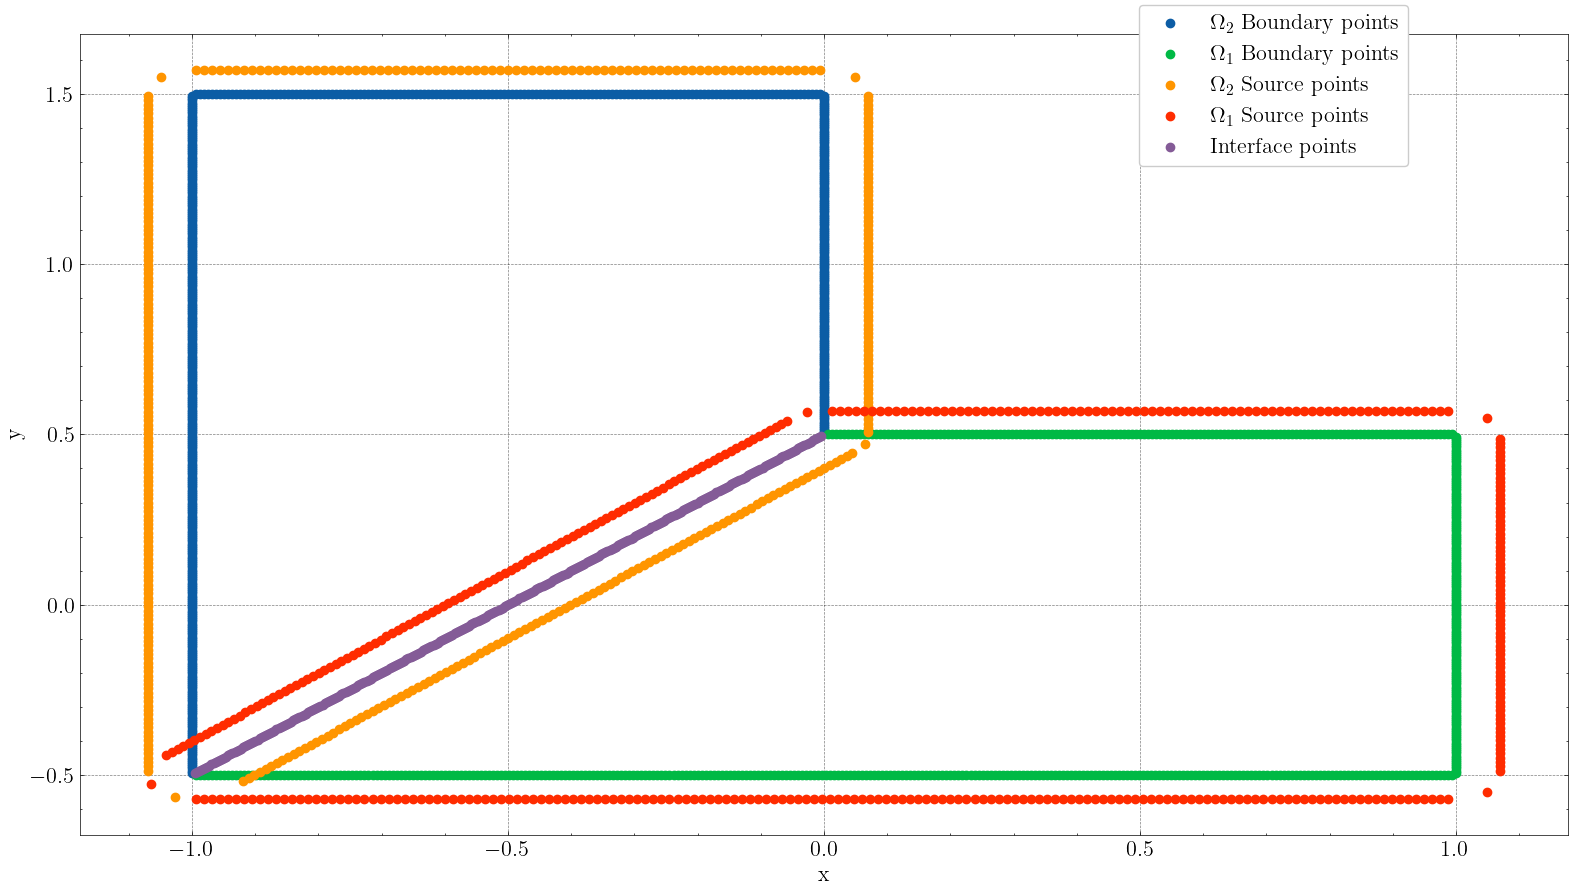
\includegraphics[height=0.4\linewidth,width=0.53\linewidth]{Images/Transmission/L_shape_2_axis_col_points.png}
    %\captionsetup{width=0.9\linewidth} % Adjust the width of the caption
    \caption{L-shape domain with the interface on the symmetry axis. Configuration of the boundary, source and interface points.}
    \label{transmission_L_shape_col_axis_config}
\end{figure}

\begin{table}[htbp]
    \centering
    \begin{tabular}{cccccc}
      \toprule
      \multirow{2}{*}{\textbf{\(k_1\) value}} & \multicolumn{2}{c}{\textbf{Boundary Error}} & \multicolumn{2}{c}{\textbf{Interface Errors}} & \multirow{2}{*}{\textbf{Condition number}} \\
      \cmidrule(lr){2-3} \cmidrule(lr){4-5}
      & \textbf{Domain 1} & \textbf{Domain 2} & \textbf{\(C^0\)} & \textbf{\(C^1\)} & \\
      \midrule
      1 & $1.812\times10^{-4}$ & $2.060\times10^{-4}$ & $7.305\times10^{-3}$ & $8.018\times10^{-5}$ & $1.050\times 10^{10}$ \\
      2 & $1.398\times10^{-4}$ & $9.729\times10^{-5}$ & $5.986\times10^{-4}$ & $5.505\times10^{-5}$ & $1.646\times 10^{10}$ \\
      5 & $7.096\times10^{-5}$ & $3.030\times10^{-5}$ & $1.528\times10^{-3}$ & $4.348\times10^{-5}$ & $3.730\times 10^{10}$ \\
      \bottomrule
    \end{tabular}
    \caption{Numerical relative error on the boundary and in the interface \(\gamma\)}
    \label{tab:transmission_results_L_shape_axis}
\end{table}

Since particular solutions will be added to the singular corners in \(\Omega_2\), one should now consider Neummann-Dirichlet particular solutions centered in the singular corner. These particular solutions have the form
\[
    w_{p_2}(r,\theta) = \alpha_{p_2} r^{\alpha_{p_2}}\cos(\alpha_{p_2}(\theta-\theta_2)),
\]
where the \(\alpha_{p_2}\) coefficients are the same as before, \(\Theta = \frac{3}{4}\pi\) and \(\theta_2=\frac{5}{4}\pi\) is the angle shift. Notice that \(\Theta\) is the same in both domains. The (polar) gradient of \(w\) is now
\begin{equation*}
    \nabla w(r,\theta)_{p_2} = \left(\frac{(2 \pi  {p_2}+\pi )^2 r^{\frac{2 \pi  {p_2}+\pi }{2 \Theta }} \cos \left(\theta +\frac{\pi  \left({p_2}+\frac{1}{2}\right) (s-\theta )}{\Theta }\right)}{4 \Theta ^2 r},\frac{(2 \pi  {p_2}+\pi )^2 r^{\frac{2 \pi  {p_2}+\pi }{2 \Theta }} \sin \left(\theta +\frac{\pi  \left({p_2}+\frac{1}{2}\right) (s-\theta )}{\Theta }\right)}{4 \Theta ^2 r}\right).
\end{equation*}

Considering the expansion \eqref{num_particular_L_shape_rect_equation} for the \(w_{p_2}\) particular solutions, one can add more blocks to the matrix \eqref{transmission_mat_L_rect_exp}. Table \ref{tab:transmission_results_L_shape_axis_particular} shows the results when particular solutions are added to both domains. Once again, negative values of \(p_2\) were considered. Without intending to show too much data (because we would have to account for every combination of \(p_1\) and \(p_2\) values), we fix \(p_2=0, 1\). The reason for this choice is that we noticed better results are achieved when increasing the number of particular solutions in the domain where the diffusion coefficient is increasing. In this case, we are only varying the coefficient \(k_1\), and therefore, we can fix the \(p_2\) values.

\begin{table}[!htbp]
    \centering
    \begin{longtable}{ccccccc}
        \toprule
        \multicolumn{1}{c}{\textbf{\(p_1\) values}} & \multicolumn{1}{c}{\textbf{\(k_1\) value}} & \multicolumn{2}{c}{\textbf{Boundary Error}} & \multicolumn{2}{c}{\textbf{Interface Errors}} & \multicolumn{1}{c}{\textbf{Condition number}} \\
        \cmidrule(lr){2-2} \cmidrule(lr){3-4} \cmidrule(lr){5-6} \cmidrule(lr){7-7}
        & & \textbf{Domain 1} & \textbf{Domain 2} & \textbf{\(C^0\)} & \textbf{\(C^1\)} & \\
        \midrule
        \endfirsthead % Header for the first page
        \multicolumn{7}{l}{{\footnotesize\emph{Continued from previous page}}} \\
        \toprule
        \multicolumn{1}{c}{\textbf{\(p\) value}} & \multicolumn{1}{c}{\textbf{\(k_1\) value}} & \multicolumn{2}{c}{\textbf{Boundary Error}} & \multicolumn{2}{c}{\textbf{Interface Errors}} & \multicolumn{1}{c}{\textbf{Condition number}} \\
        \cmidrule(lr){2-2} \cmidrule(lr){3-4} \cmidrule(lr){5-6} \cmidrule(lr){7-7}
        & & \textbf{Domain 1} & \textbf{Domain 2} & \textbf{\(C^0\)} & \textbf{\(C^1\)} & \\
        \midrule
        \endhead % Header for subsequent pages
        \midrule[\heavyrulewidth] % Horizontal line
        \multicolumn{7}{r}{{\footnotesize\emph{Continued on next page}}} \\
        \endfoot % Footer for subsequent pages
        \bottomrule
        \endlastfoot % Footer for the last page
        
        % Data for p = [0, 1]
        0, 1 & 1 & $3.107\times10^{-7}$ & $2.100\times10^{-7}$ & $1.158\times10^{-5}$ & $1.019\times10^{-7}$ & $1.054\times10^{10}$ \\
        & 2 & $1.061\times10^{-7}$ & $6.892\times10^{-7}$ & $6.366\times10^{-5}$ & $7.065\times10^{-8}$ & $1.648\times10^{10}$ \\
        & 5 & $1.207\times10^{-7}$ & $1.141\times10^{-6}$ & $9.544\times10^{-5}$ & $9.487\times10^{-8}$ & $3.732\times10^{10}$ \\
        \midrule[\heavyrulewidth] % Horizontal line
        
        % Data for p = [-1, 0, 1]
        -1, 0, 1 & 1 & $3.319\times10^{-7}$ & $2.026\times10^{-7}$ & $1.813\times10^{-5}$ & $1.048\times10^{-7}$ & $1.054\times10^{10}$ \\
        & 2 & $1.676\times10^{-7}$ & $3.166\times10^{-7}$ & $8.375\times10^{-6}$ & $7.951\times10^{-8}$ & $1.647\times10^{10}$ \\
        & 5 & $9.871\times10^{-8}$ & $4.807\times10^{-7}$ & $1.549\times10^{-6}$ & $5.285\times10^{-8}$ & $3.732\times10^{10}$ \\
        \midrule[\heavyrulewidth] % Horizontal line

        % Data for p = [-2, -1, 0, 1]
        -2, -1, 0, 1 & 1 & $3.070\times10^{-7}$ & $2.415\times10^{-7}$ & $1.610\times10^{-5}$ & $9.893\times10^{-8}$ & $5.659\times10^{12}$ \\
        & 2 & $1.762\times10^{-7}$ & $2.670\times10^{-7}$ & $8.385\times10^{-6}$ & $8.480\times10^{-8}$ & $5.656\times10^{12}$ \\
        & 5 & $9.761\times10^{-8}$ & $3.201\times10^{-7}$ & $1.993\times10^{-6}$ & $6.049\times10^{-8}$ & $5.655\times10^{12}$ \\
        \midrule[\heavyrulewidth] % Horizontal line
    \end{longtable}
    \caption{Numerical relative error on the boundary and in the interface \(\gamma\) after considering particular (angular) solutions}
    \label{tab:transmission_results_L_shape_axis_particular}
\end{table}

Again, we found the same surprising results as before, where considering negative values for \(p_1\) achieves better approximations, particularly when \(k_1 \neq k_2 = 1\). An interesting observation was made when considering negative values for \(p_2\): in that case, if \(p_1\) is also negative, the solution in both domains would explode. Intuitively, one can treat the problem numerically as an exterior problem in only one domain. On the other hand, one may consider \(p_1 = p_2 = 0, \dots, P\), where \(P=P_1=P_2\), for \(P > 1\) (\(P\) may be as large as 8, for example, with 16 particular solutions being added in total) and the results can be as good as the ones presented in Table \ref{tab:transmission_results_L_shape_axis_particular} for \(p_1=-2, -1, 0, 1\), but only if \(k_1=k_2=1\); otherwise, the approximation on the interface gets worse than what we found. 

\begin{figure}[!htb]
    \centering
    \begin{minipage}{.5\textwidth}
      \centering
      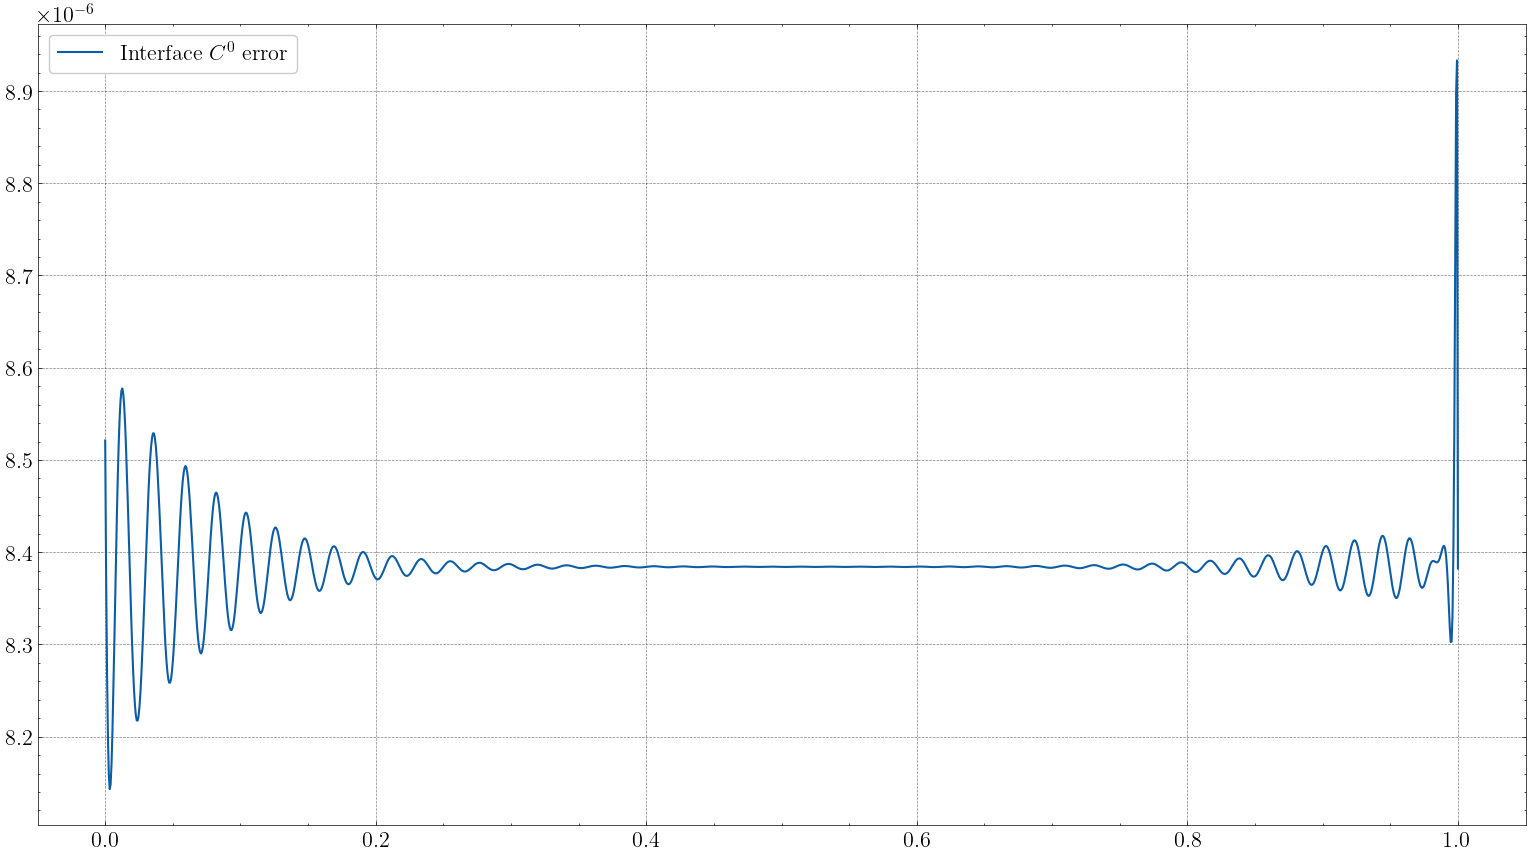
\includegraphics[width=1\linewidth]{Images/Transmission/L_shape_2_axis_c0_error_k1_2_enr.png}
      \caption{Interface \(C^0\) error}
      \label{transmission_L_axis_error_c0_k1_2}
    \end{minipage}%
    \begin{minipage}{.5\textwidth}
      \centering
      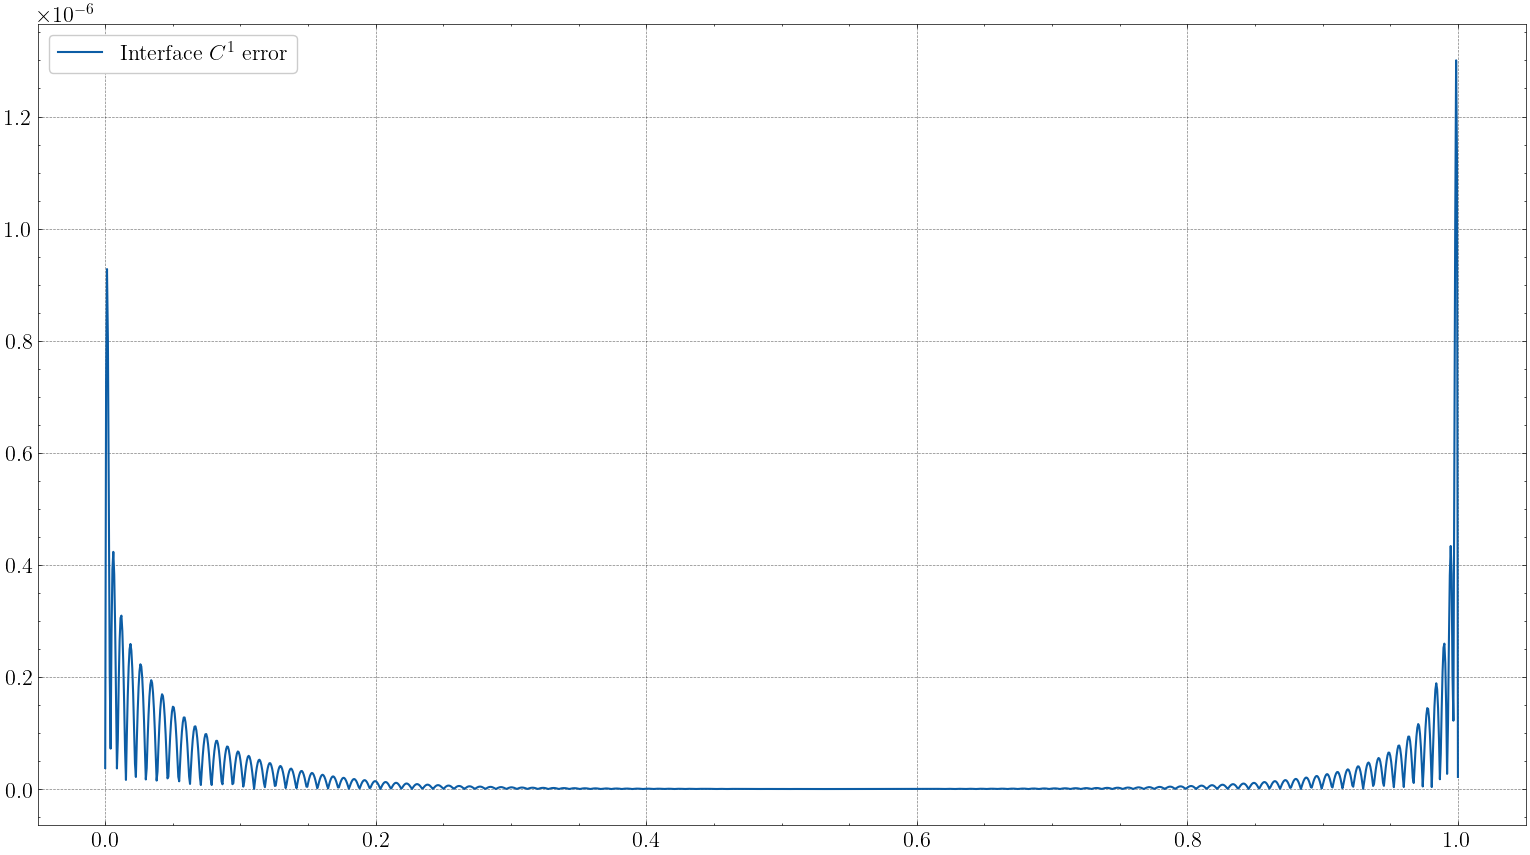
\includegraphics[width=1\linewidth]{Images/Transmission/L_shape_2_axis_c1_error_k1_2_enr.png}
      \caption{Interface \(C^0\) error}
      \label{transmission_L_axis_error_c1_k1_2}
    \end{minipage}
    
    \vspace{0.5cm} % Add some vertical space between the rows of figures
    
    \begin{minipage}{.6\textwidth}
      \centering
      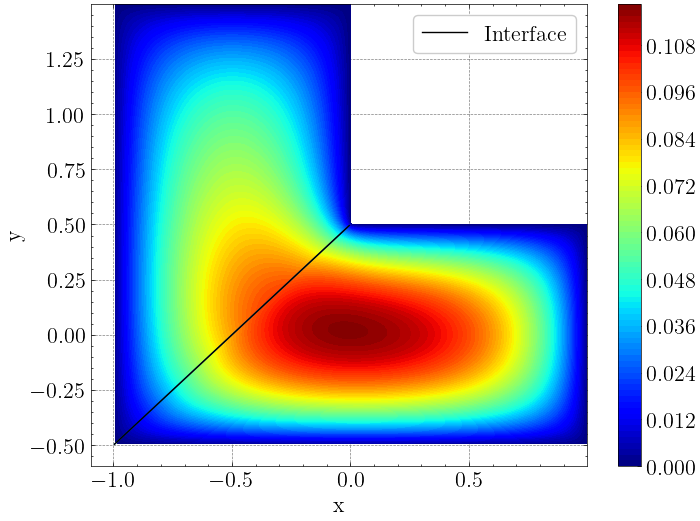
\includegraphics[width=\linewidth]{Images/Transmission/L_shape_2_axis_sol_k1_2_enr.png}
      %\caption{Numerical approximation}
      \label{transmission_L_axis_plot_k1_2}
    \end{minipage}
    
    \caption*{Absolute value of the interface errors and numerical approximation for \(k_1=2\), \(p_1=-2, -1, 0, 1\) and \(p_2 = 0, 1\).}
    \label{}
\end{figure}

Figures \ref{transmission_L_axis_error_c0_k1_2} and \ref{transmission_L_axis_error_c1_k1_2} show the absolute value of the errors for each interface point, with \(k_1=2\) and the \(p\) values for the particular solutions are \(p_1=-2, -1, 0, 1\) and \(p_2 = 0, 1\). As expected, both errors peak near the edges of the interface with special evidence when near the singular corner.